\livelloA{One-way analysis of variance}

\livelloB{Quality of car seats}

\begin{frame}
  \begin{description}
    \item[Data: ]carseat.txt \\ 
    \item[Description: ]
      \begin{footnotesize}
        \begin{itemize}
          \item \textit{Operator}: identifies which operator performed the measurement (factor);
          \item \textit{Strength}: identifies the breaking load of the fabric (in kg).
        \end{itemize}
      \end{footnotesize}
    \item[Aims: ]
      \begin{footnotesize}
        Three quality inspectors, which control the resistance of the fabric of car seats, want to conduct a reproducibility study. The aim is to check if there are differences in observed measurements due to the operator that perform the measurement.   
        \begin{itemize}
          \item[-] Let us draw the BW plot of \textit{Strength} for each operator.
          \item[-] Let us check that the different groups belong to a normally distributed population.
          \item[-] Let us check that the different groups have the same variance (homoskedasticity).
          \item[-] Let us check if there are differences between the averages of different groups.
        \end{itemize}
      \end{footnotesize}
  \end{description}
\end{frame}

\begin{frame}
  B-W Graphics of \textit{Strength} separately for each operator:\\
  \begin{center}
    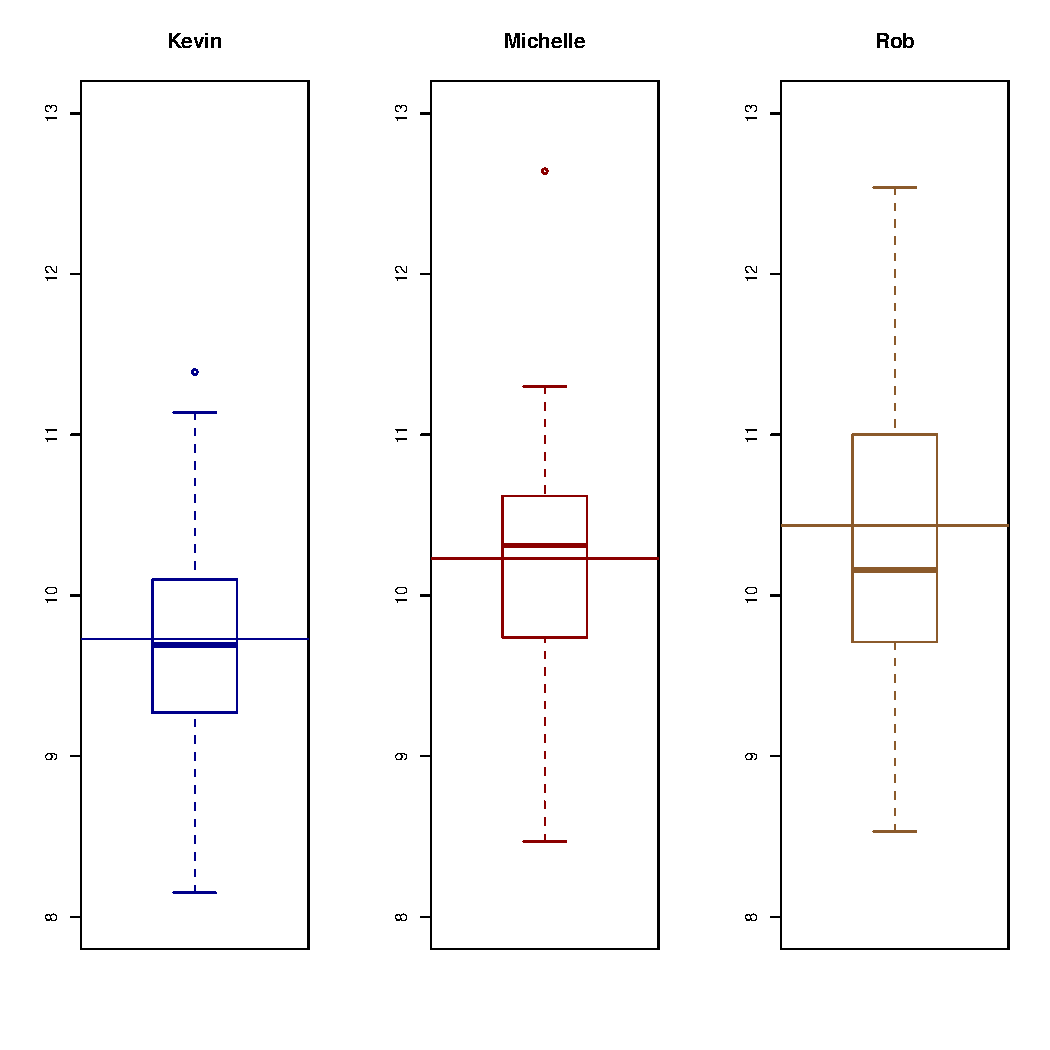
\includegraphics[width=7.5cm]{99_05_bwStrength.pdf}
  \end{center}
\end{frame}

\begin{frame}
  \vspace{0.25cm}
  The p-values of the Anderson-Darling normality test on operators are:
  \begin{itemize}
    \item Rob: 0.371;
    \item Kevin: 0.975;
    \item Michelle: 0.419.
  \end{itemize}
  \vspace{1cm}
  For each $ \alpha $ between those normally used, It is not possible to establish that data don't belong to a normally distributed population.\\
  \vspace{0.5cm}
  It is possible to assert that \textbf{the normality assumption required by ANOVA is satisfied}.
\end{frame}

\begin{frame}
  \vspace{0.25cm}
  One of the assumption of ANOVA is that different groups have variance equal between them. The hypothesis for this test are:\\ 
  $ H_0 $: all operators have the same variance;\\
  $ H_A $: almost one operator has variance different from others.\\
  \vspace{0.5cm}
  Both Bartlett test (p-value = 0.301) and Levene test (p-value = 0.400) show that the variances are not significantly different.\\
  \vspace{0.5cm}
  This fact means that the observed differences in the variances of groups are due to chance alone, so  \textbf{the homoskedasticity assumption required by ANOVA is satisfied}.
\end{frame}

\begin{frame}[fragile]
  \vspace{0.25cm}
  The variance analysis gives the following result:
  \begin{verbatim}
             Df  Sum Sq  Mean Sq  F value  p value  
Operator     2    6.621   3.3104   3.8508  0.02577
Residuals   72   61.895   0.8597  
  \end{verbatim}
  F test is the ratio between MS of Operatore factor and residuals (or error).\\
  \vspace{0.25cm}
  An $ F $ value close to 1 means that the differences in the averages of the factors are not significant but they can be due to chance.\\
  \vspace{0.25cm}
  The ratio $ F $ is distributed as a random variable F with 2 and 72 degrees of freedom.\\
\end{frame}

\begin{frame}
  \vspace{0.75cm}
  The p-value is 2.577\%.  It gives different conclusion according to the fixed significance level $ \alpha $:
  \vspace{0.5cm}
  \begin{itemize}
    \item The null hypothesis asserts that the averages are all equal and the alternative hypothesis asserts that \textbf{at least one of the averages is different}. Considering a 5\% confidence level, the null hypothesis $ H_0 $ is rejected;
    \vspace{0.5cm}
    \item Considering a 1\% confidence level, instead, the null hypothesis is not rejected. The conclusion is that the averages are  \textbf{statistically equal to each other}.
  \end{itemize}
\end{frame}

\begin{frame}
  \vspace{1cm}
  Since, at least for $ \alpha = 0.05 $, the averages of the groups seem to be all equal to each other, It can be useful apply the contrasts to analyse the differences between different operators.\\ 
  \vspace{1cm}
  It only makes sense if Rob, Kevin e Michelle are the only operators of the company and so we are applying a \textbf{fixed effects ANOVA}.
\end{frame}

\begin{frame}
  Graphical check of the model:\\
  \vspace{.1cm}
  \begin{center}
    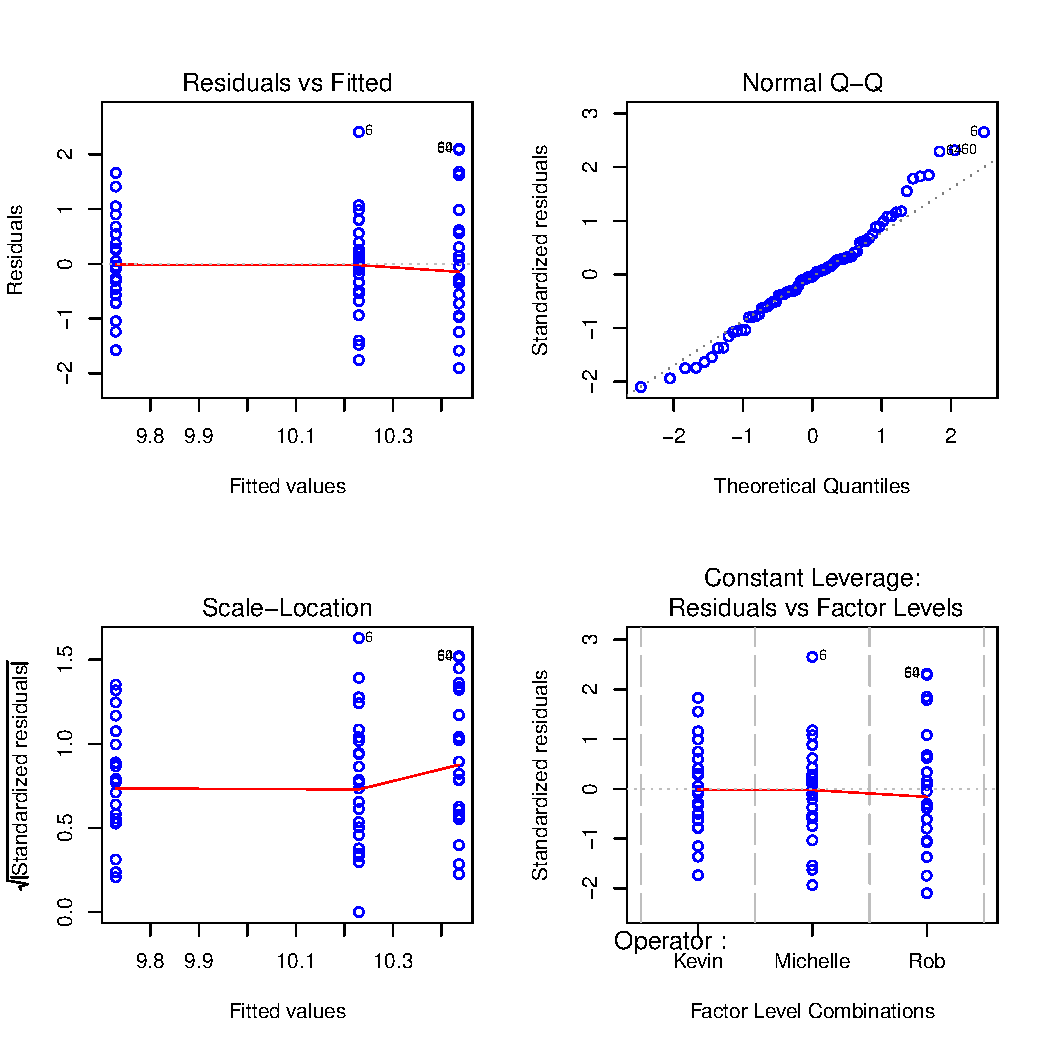
\includegraphics[width=7.5cm]{99_05_residAnovaCarseat}
    \end{center}
\end{frame}

\livelloB{Multi-head machine}

\begin{frame}
  \begin{description}
    \item[Data: ]pencap.txt \\ 
    \item[Description: ]
      \begin{footnotesize}
        \begin{itemize}
          \item \textit{Cavity}: indicates the number of head (factor);
          \item \textit{Width}: indicates the measurement (in mm).
        \end{itemize}
      \end{footnotesize}
    \item[Aims: ]
      \begin{footnotesize}
        A society that produces ballpoint pens uses a multi-head machine for the production of caps for pens. The productor wants to compare the means and the variances on all 16 heads and to determine if there are variations on the means of the different heads.
        \begin{itemize}
          \item[-] Let us show the BW plot of \textit{Width} for each head.
          \item[-] Let us check if different groups belong to a normally distributed population.
          \item[-] Let us check if the different groups have the same variance (homoskedasticity).
          \item[-] Let us check if there are differences between the means of the different groups.
        \end{itemize}
      \end{footnotesize}
  \end{description}
\end{frame}

\begin{frame}
  B-W Graph of \textit{Width} separately for each head:\\
  \vspace{-0.5cm}
  \begin{center}
    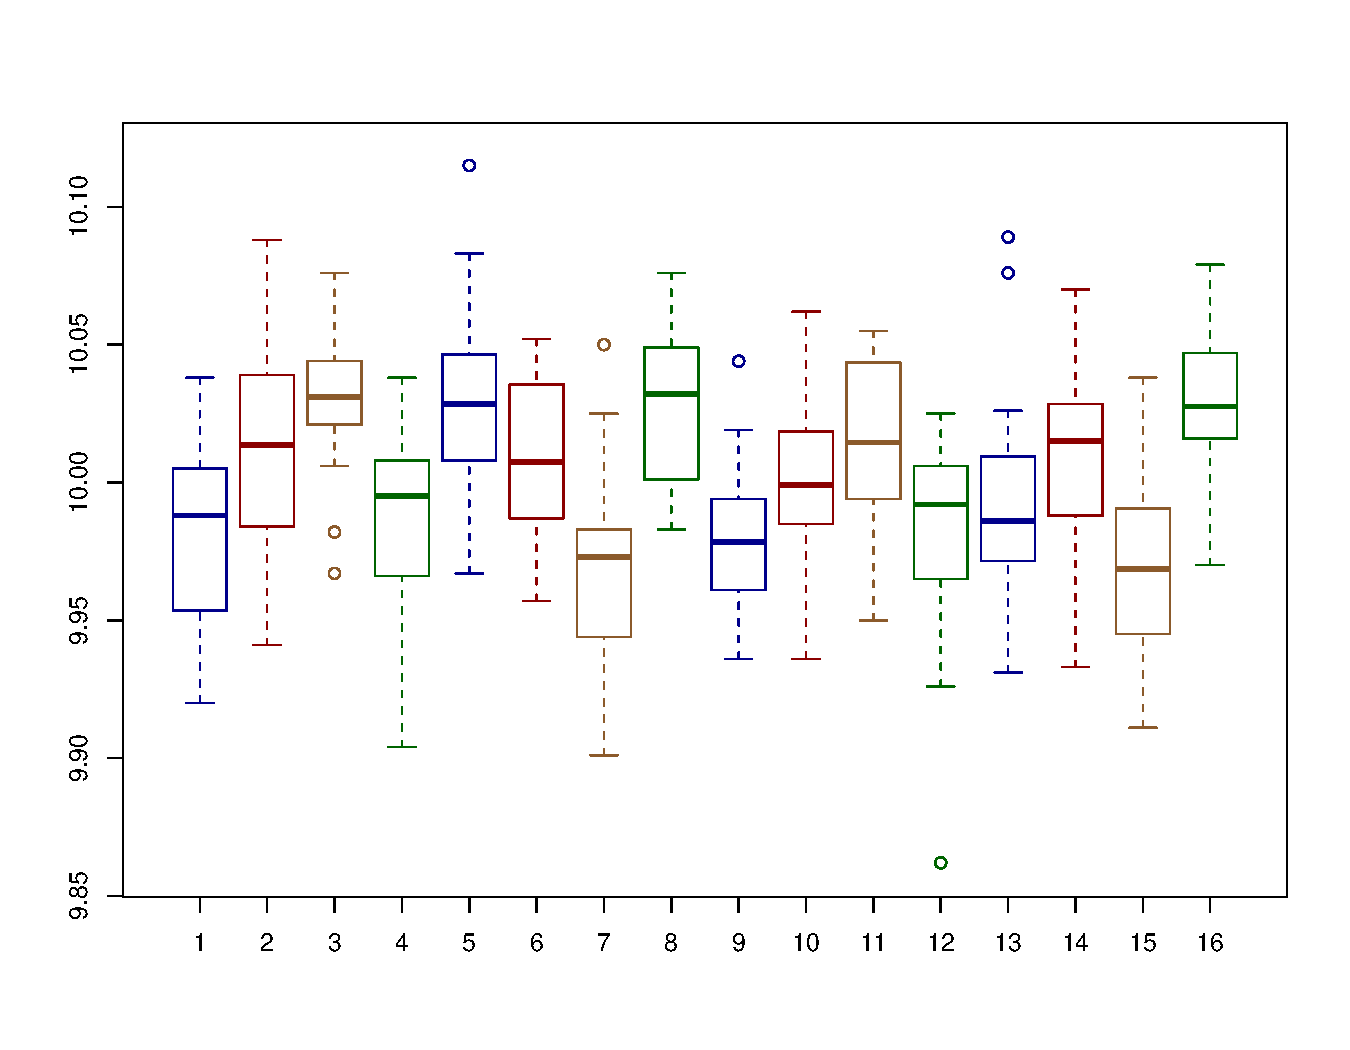
\includegraphics[width=11cm]{99_05_bwPencap.pdf}
  \end{center}
\end{frame}

\begin{frame}
  \begin{minipage}[t]{0.48\textwidth}
    Normality\\

    \vspace*{0.25cm}
    Anderson-Darling Test:
    \begin{table}[ht]
      \begin{tiny}
        \begin{tabular}{lr}
          \hline
          Cavity & p value \\ 
          \hline
           1 & 0.2155 \\ 
           2 & 0.9142 \\ 
           3 & 0.3541 \\ 
           4 & 0.1333 \\ 
           5 & 0.5674 \\ 
           6 & 0.3454 \\ 
           7 & 0.2569 \\ 
           8 & 0.5680 \\ 
           9 & 0.8530 \\ 
          10 & 0.6430 \\ 
          11 & 0.5147 \\ 
          12 & 0.0264 \\ 
          13 & 0.0845 \\ 
          14 & 0.5149 \\ 
          15 & 0.5856 \\ 
          16 & 0.2628 \\ 
          \hline
        \end{tabular}
      \end{tiny}
    \end{table}
  \end{minipage}
  \hfill
  \begin{minipage}[t]{0.48\textwidth}
    Homoskedasticity of variances\\

    \vspace*{0.25cm}
    Bartlett Test:\\
    \texttt{p value: 0.726}\\

    \vspace*{0.75cm}
    Levene Test:\\
    \texttt{p value: 0.899}\\
  \end{minipage}
\end{frame}

\begin{frame}[fragile]
  \vspace{0.25cm}
  Variance analysis:
  \begin{verbatim}
             Df  Sum Sq   Mean Sq F value   p value    
Cavity       15 0.14199 0.0094659  8.3501 5.922e-16
Residuals   304 0.34462 0.0011336    
  \end{verbatim}
\end{frame}

\begin{frame}
  Graphical check of the model:\\
  \vspace{.1cm}
  \begin{center}
    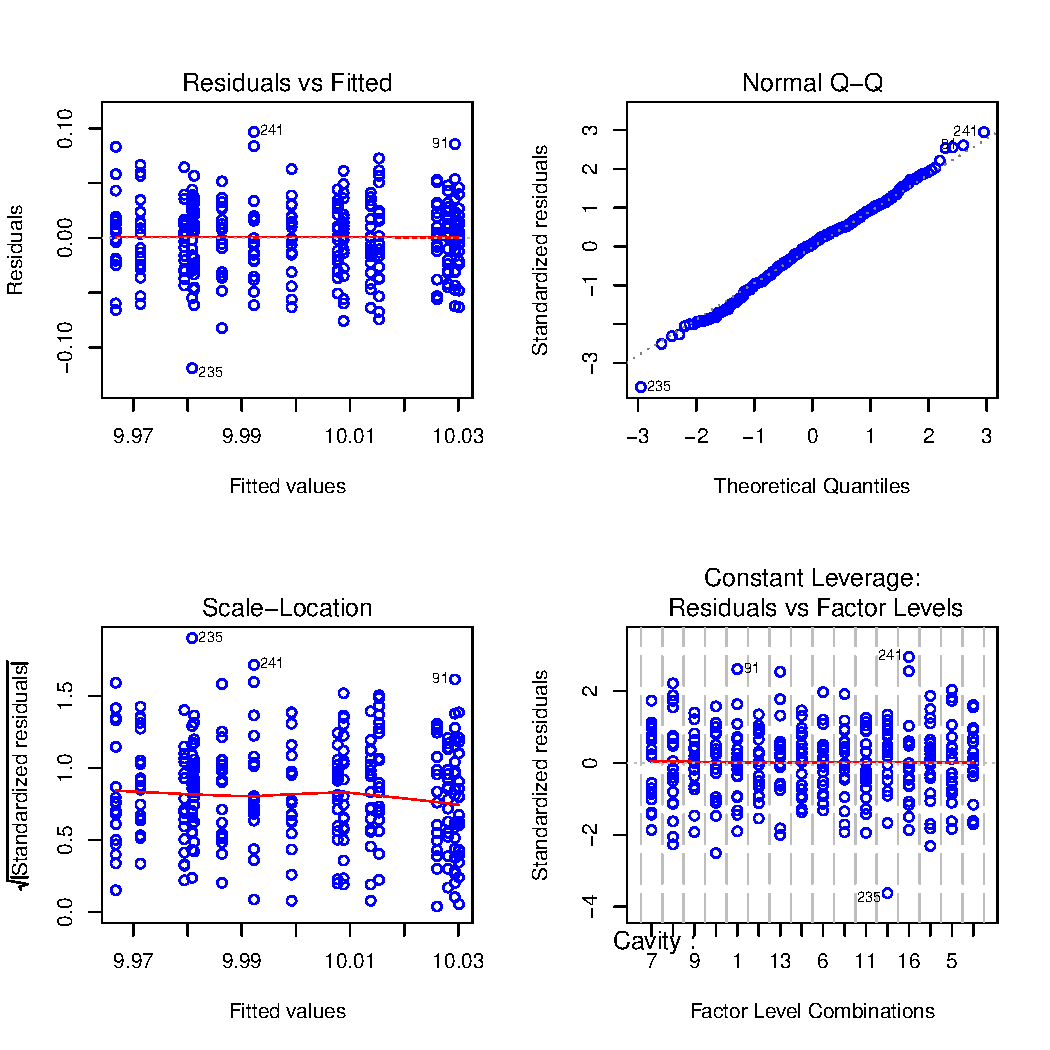
\includegraphics[width=7.5cm]{99_05_residAnovaPencap}
    \end{center}
\end{frame}

\livelloB{Tear resistance}

\begin{frame}
  \begin{description}
    \item[Data: ]sturdy.txt \\ 
    \item[Description: ]
      \begin{footnotesize}
        \begin{itemize}
          \item \textit{Time}: indicates the time between the solicitation and the tear (in minutes);
          \item \textit{Group}: indicates the raincoats brand (factor).
        \end{itemize}
      \end{footnotesize}
    \item[Aims: ]
      \begin{footnotesize}
        The aim is to study the tear resistance of five different raincoats brand. The raincoats were subjected to the same solicitation, and the time between the solicitation and the tear (in minutes and in decimal fractions of a minute) was measured.   
        \begin{itemize}
          \item[-] Let us show the BW plot of \textit{Time} for each brand.
          \item[-] Let us check that different groups belong to a normally distributed population.
          \item[-] Let us check if the different groups have the same variance (homoskedasticity).
          \item[-] Let us check if there are differnces between thwe means of the different groups.
        \end{itemize}
      \end{footnotesize}
  \end{description}
\end{frame}

\begin{frame}
  B-W Graph of \textit{Time} separately for each brand:\\
  \vspace{-0.5cm}
  \begin{center}
    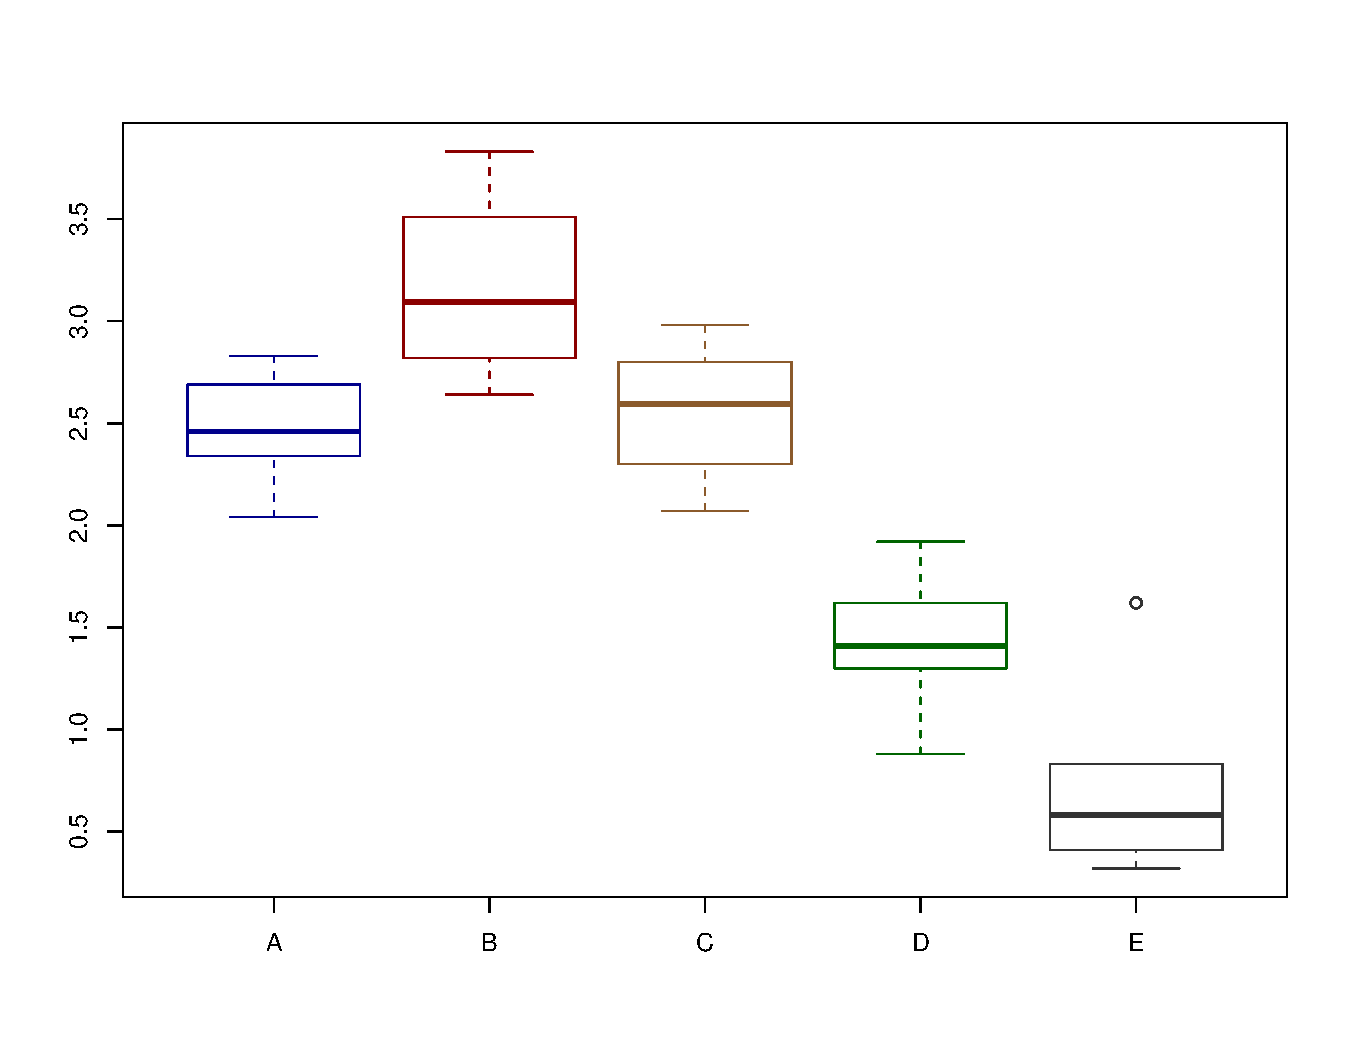
\includegraphics[width=11cm]{99_05_bwSturdy.pdf}
  \end{center}
\end{frame}

\begin{frame}
  Normality\\
  \vspace*{0.25cm}
  Because of the low number of units within each groups, It is not possible to perform Anderson Darling test. However, analysing the B-W plot of the previous slide, the normality assumption is considered valid. \\ 
  \vspace{1cm}
  Homoskedasticity of variances\\
  \vspace*{0.25cm}
  Bartlett Test\\
  \texttt{p value: 0.7722}\\
  \vspace*{0.75cm}
  Levene Test\\
  \texttt{p value: 0.9214}\\
\end{frame}

\begin{frame}[fragile]
  \vspace{0.25cm}
  Variance analysis:
  \begin{verbatim}
            Df  Sum Sq Mean Sq F value   p value    
Group        4 18.1681  4.5420  28.261 3.475e-08
Residuals   21  3.3751  0.1607       
  \end{verbatim}
\end{frame}

\begin{frame}
  Graphical check of the model:\\
  \vspace{.1cm}
  \begin{center}
    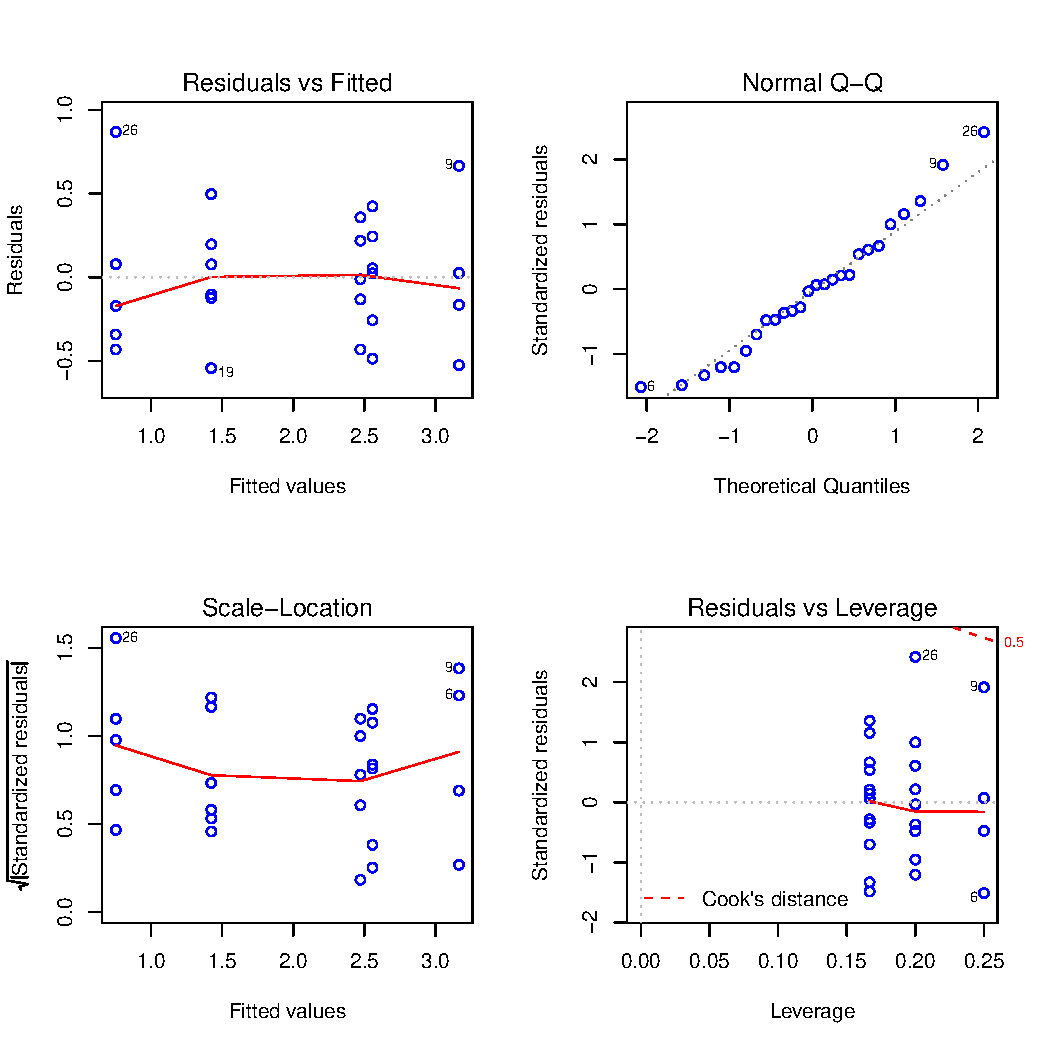
\includegraphics[width=7.5cm]{99_05_residAnovaSturdy}
    \end{center}
\end{frame}

\livelloB{Effect of toxic agent}

\begin{frame}
  \begin{description}
    \item[Data: ]rats.txt \\ 
    \item[Description: ]
      \begin{footnotesize}
        \begin{itemize}
          \item \textit{Time}: identifies the survival time (in tens of hours);
          \item \textit{Poison}: identifies the poison type (factor);
          \item \textit{Treatment}: identifies the type of treatment (factor).
        \end{itemize}
      \end{footnotesize}
    \item[Aims: ]
      \begin{footnotesize}
        The aim is to study the survival time to different types of rats treatments to which has been administered the second type of poison.  
        \begin{itemize}
          \item[-] Let us show the BW plot of \textit{Time} for each treatment.
          \item[-] Let us check if the different groups belong to a normally distributed population.
          \item[-] Let us check if the different groups have the same variance (homoskedasticity).
          \item[-] Is It posible to make a comparison? How?
        \end{itemize}
      \end{footnotesize}
  \end{description}
\end{frame}

\begin{frame}
  B-W Graph of \textit{Time} separately for each treatment:\\
  \vspace{-0.5cm}
  \begin{center}
    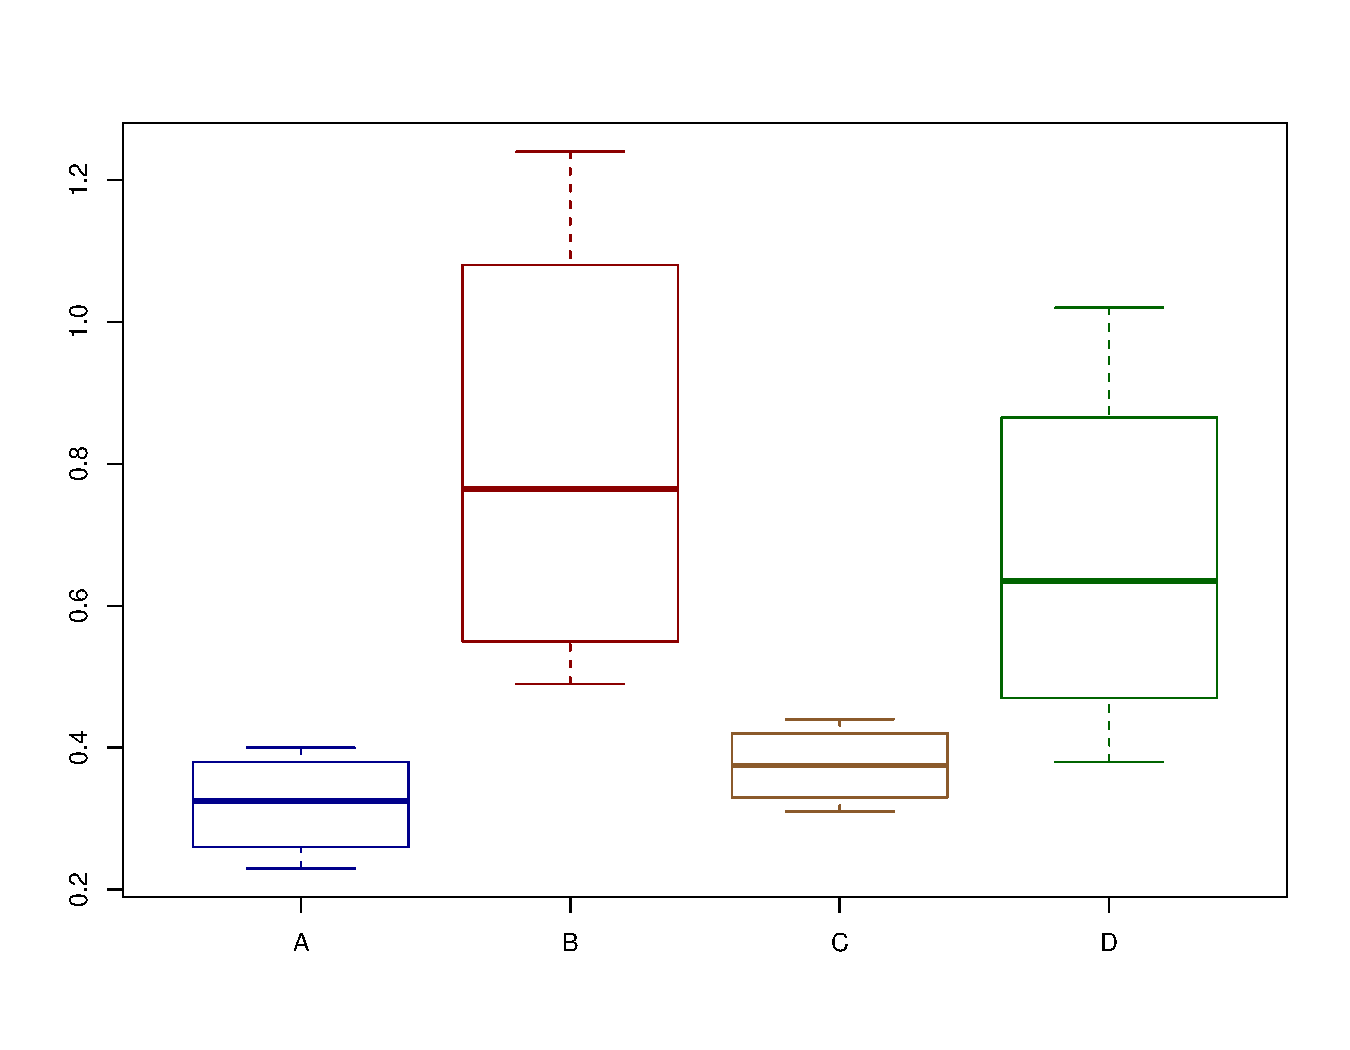
\includegraphics[width=11cm]{99_05_bwTreatment.pdf}
  \end{center}
\end{frame}

\begin{frame}
  Normality\\
  \vspace*{0.25cm}
  Because of the low number of units within each group, It is not possible to perform Anderson Darling test. However, analysing the B-W plot of the previous slide, the normality assumption is considered valid. \\ 
  \vspace{1cm}
  Homoskedasticity of variances\\
  \vspace*{0.25cm}
  Bartlett Test - \texttt{p value: 0.0229}\\
  Levene Test - \texttt{p value: 0.0373}\\
  \vspace*{0.75cm}
  The homoskedasticity hypothesis is rejected with a 5\% confidence level.
\end{frame}

\begin{frame}
  B-W graph of the reciprocal of \textit{Time} for each treatment:\\
  \vspace{-0.5cm}
  \begin{center}
    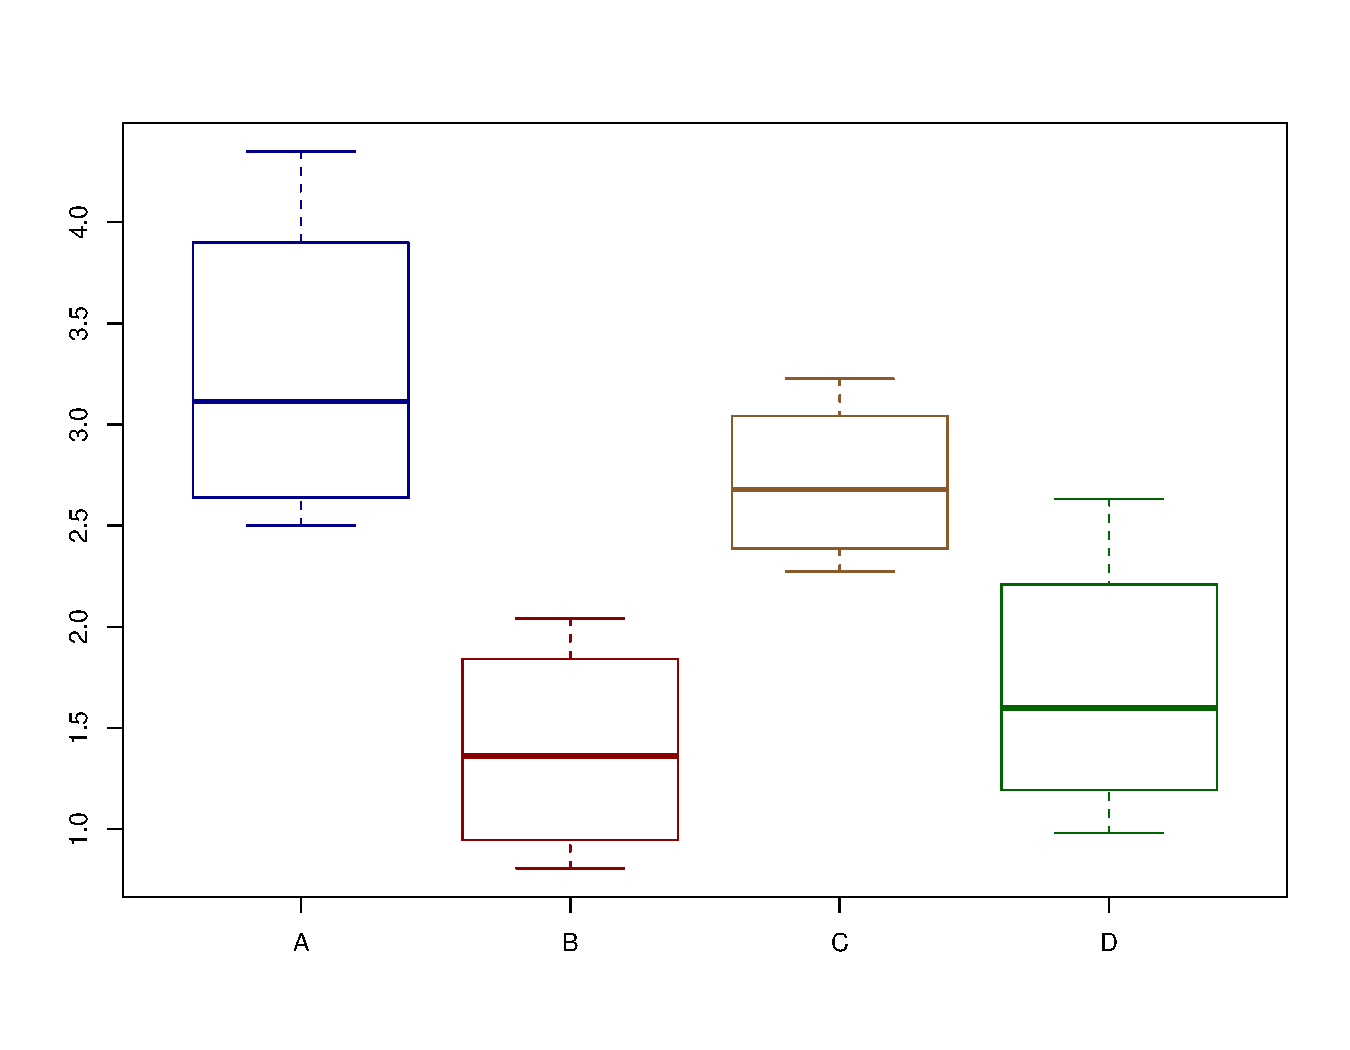
\includegraphics[width=11cm]{99_05_bwInvTreatment.pdf}
  \end{center}
\end{frame}

\begin{frame}
  Normality\\
  \vspace*{0.25cm}
  Because of the low number of units within each group, It is not possible to perform Anderson Darling test. However, analysing the B-W plot of the previous slide, the normality assumption is considered valid. \\ 
  \vspace{1cm}
  Homoskedasticity of variances\\
  \vspace*{0.25cm}
  Bartlett Test:\\
  \texttt{p value: 0.7337}\\
  \vspace*{0.75cm}
  Levene Test:\\
  \texttt{p value: 0.6244}\\
\end{frame}

\begin{frame}[fragile]
  \vspace{0.25cm}
  Variance analysis:
  \begin{verbatim}  
            Df Sum Sq Mean Sq F value  p value  
Treatment    3 9.1424 3.04747  7.3913 0.004594
Residuals   12 4.9477 0.41231       
  \end{verbatim}
\end{frame}

\begin{frame}
   Graphical check of the model:\\
  \vspace{.1cm}
  \begin{center}
    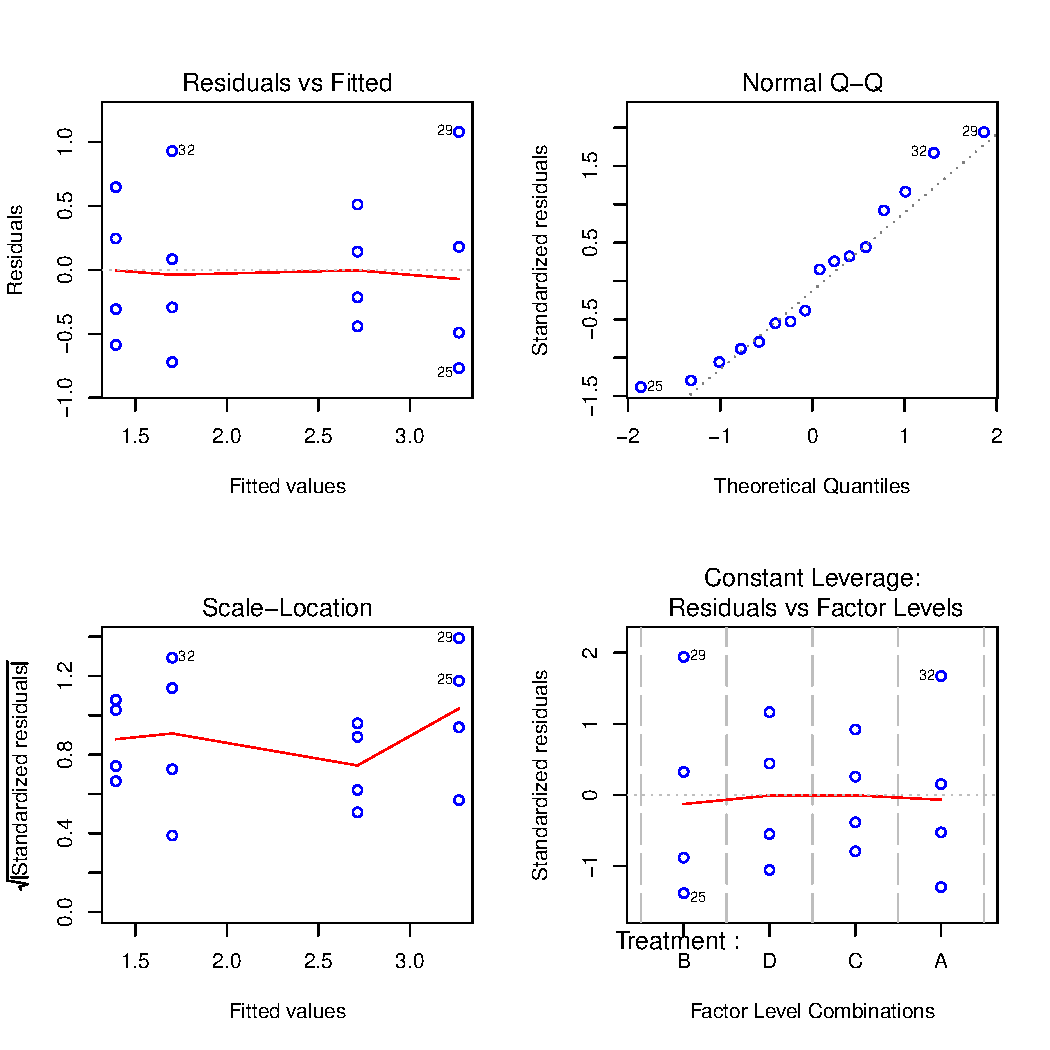
\includegraphics[width=7.5cm]{99_05_residAnovaInvTreatment}
    \end{center}
\end{frame}



\livelloA{Multi-factor variance analysis}

\livelloB{Stopping distance of a car on wet road}

\begin{frame}
  \begin{description}
    \item[Data: ]brakedis.txt \\ 
    \item[Description: ]
      \begin{footnotesize}
        \begin{itemize}
          \item \textit{Tire}: identifies the tyre model (factor);
          \item \textit{Tread}: identifies the tread depth, 1.5 or 10.0 mm (factor);
          \item \textit{ABS}: indicates whether the ABS is in operation (factor);
          \item \textit{Distance}: indicates the distance traveled, on wet surfaces, by the vehicle before stopping (in meters). 
        \end{itemize}
      \end{footnotesize}
    \item[Aims: ]
      \begin{footnotesize}
        The engineers want to know if the distance traveled by a car on wet surfaces is influenced by the tyre model, by the wear of the tread, the operation or not of the ABS. Data are collected with the same car at the speed of 60 km/h before braking.
      \begin{itemize}
          \item[-] Let us check which factors influence the stopping distance on wet surfaces.
        \end{itemize}
      \end{footnotesize}
  \end{description}
\end{frame}

\begin{frame}[fragile]
  \vspace{0.25cm}
  The first model analysed includes all factors and all possible interactions. The model is indicated in the following way:
  $ Distance = Tire \; | \; Tread \; | \; ABS $.\\
  The variance analysis produces the following result:
  \begin{verbatim}
               Df  Sum Sq Mean Sq F value   p value    
Tire            2  37.316  18.658  9.4074  0.003488
Tread           1   0.107   0.107  0.0538  0.820517    
ABS             1 140.167 140.167 70.6723 2.255e-06
Tire:Tread      2   6.656   3.328  1.6779  0.227740    
Tread:ABS       1   1.215   1.215  0.6126  0.448979    
Tire:ABS        2   2.986   1.493  0.7527  0.492074    
Tire:Tread:ABS  2   2.572   1.286  0.6485  0.540199    
Residuals      12  23.800   1.983 
  \end{verbatim}
\end{frame}

\begin{frame}[fragile]
  \vspace{0.25cm}
  Only two coefficient of the previous model are significant.\\ 
  \vspace{0.5cm}
  By eliminating a term at a time, starting from that with the higher p-value, we arrive at the following reduced model:
  \begin{verbatim}
            Df  Sum Sq Mean Sq F value   p value 
Tire         2  37.316  18.658  9.9946 0.0009792
ABS          1 140.167 140.167 75.0843 3.322e-08
Residuals   20  37.336   1.867  
  \end{verbatim}
  So, It is possible to conclude that the stopping distance is influenced by the tyre model and by the operation of ABS.
\end{frame}

\begin{frame}
   Graphical check of the model:\\
  \vspace{.1cm}
  \begin{center}
    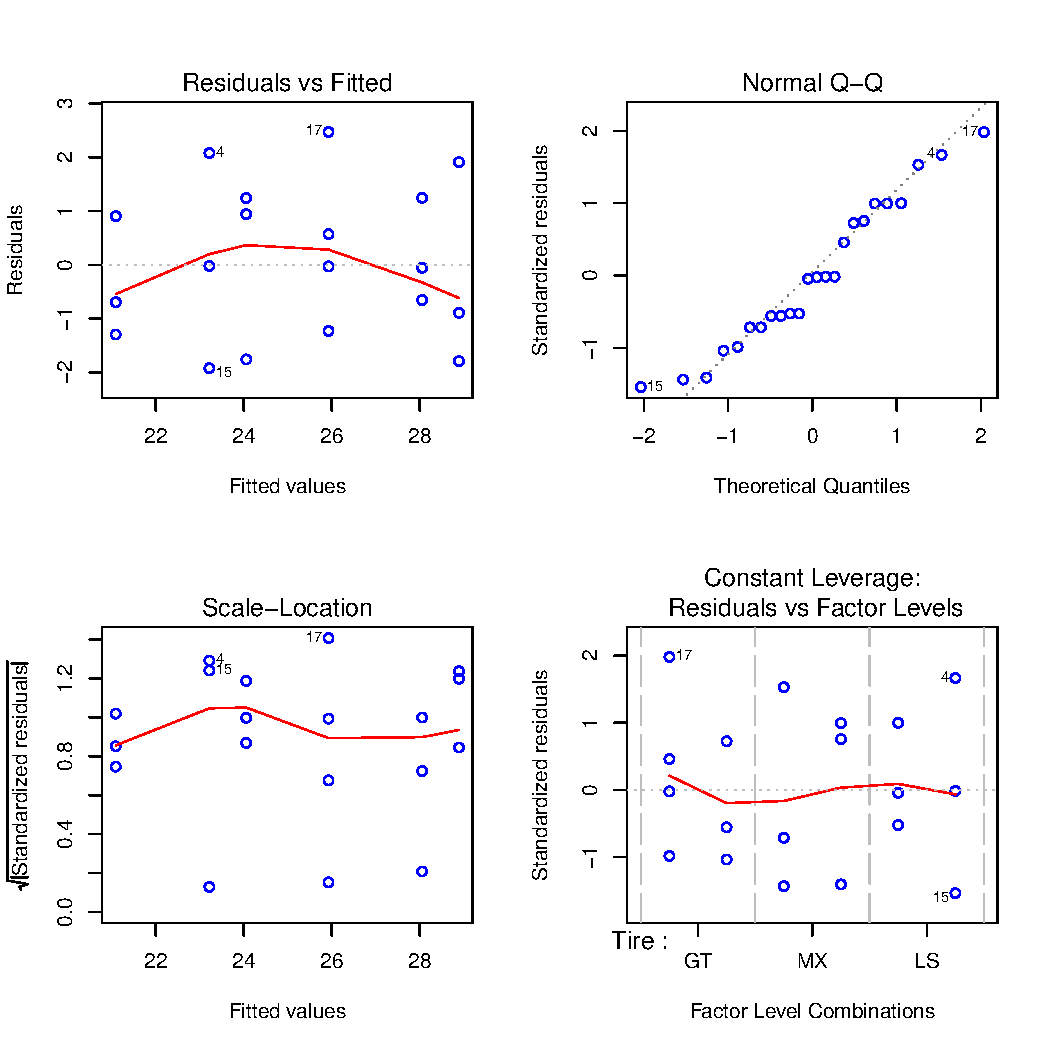
\includegraphics[width=7.5cm]{99_05_residAnovaBrakedis}
    \end{center}
\end{frame}

\livelloB{Wine quality}

\begin{frame}
  \begin{description}
    \item[Data: ]rioja.txt \\ 
    \item[Description: ]
      \begin{footnotesize}
        \begin{itemize}
          \item \textit{Judge}: indicates the name of the taster (factor);
          \item \textit{Wine}: indicates the wine name (factor);
          \item \textit{Trial}: indicates the order of tasting;
          \item \textit{Score}: indicates the evaluation reached (score).
        \end{itemize}
      \end{footnotesize}
    \item[Aims: ]
      \begin{footnotesize}
        A society wants to determine if there are significant differences in the quality of three types of wine: Matador, Conquistador e Saeta. Ten judges have assigned a score to the wine tasted. The order of tasting was random.
      \begin{itemize}
          \item[-] Let us perform a variance analysis to check if the mean of the score is equal for all types of wine.
          \item[-] Let us perform a variance analysis to check if the mean of the score is equal for all the judges.
          \item[-] Let us perform a variance analysis to check if the mean of the score depends by the type of wine and by the judge.
        \end{itemize}
      \end{footnotesize}
  \end{description}
\end{frame}

\begin{frame}
  B-W Graph of \textit{Score} separately for each type of wine:\\
  \begin{center}
    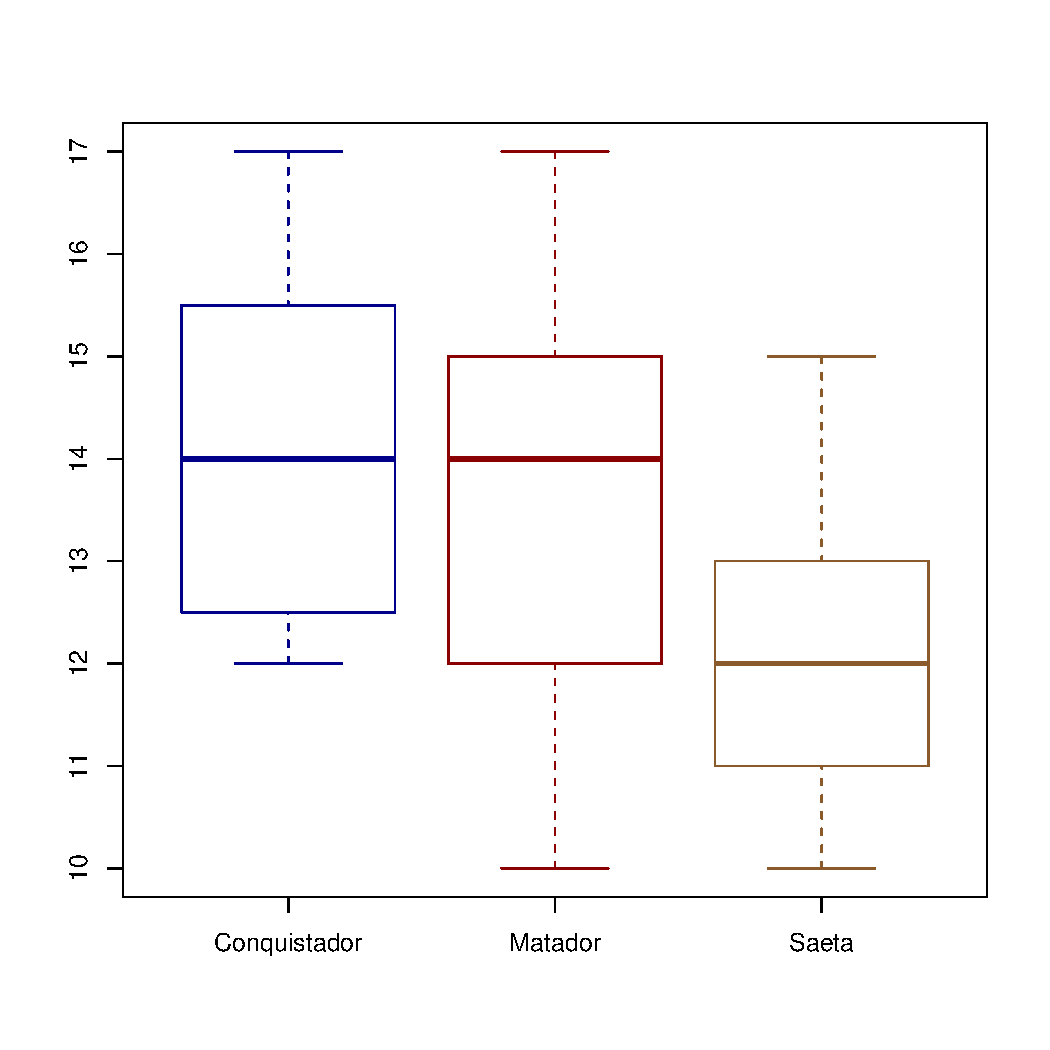
\includegraphics[width=7.5cm]{99_05_bwWine.pdf}
  \end{center}
\end{frame}

\begin{frame}
  B-W Graph of \textit{Score} separately for each judge:\\
  \vspace{-1cm}
  \begin{center}
    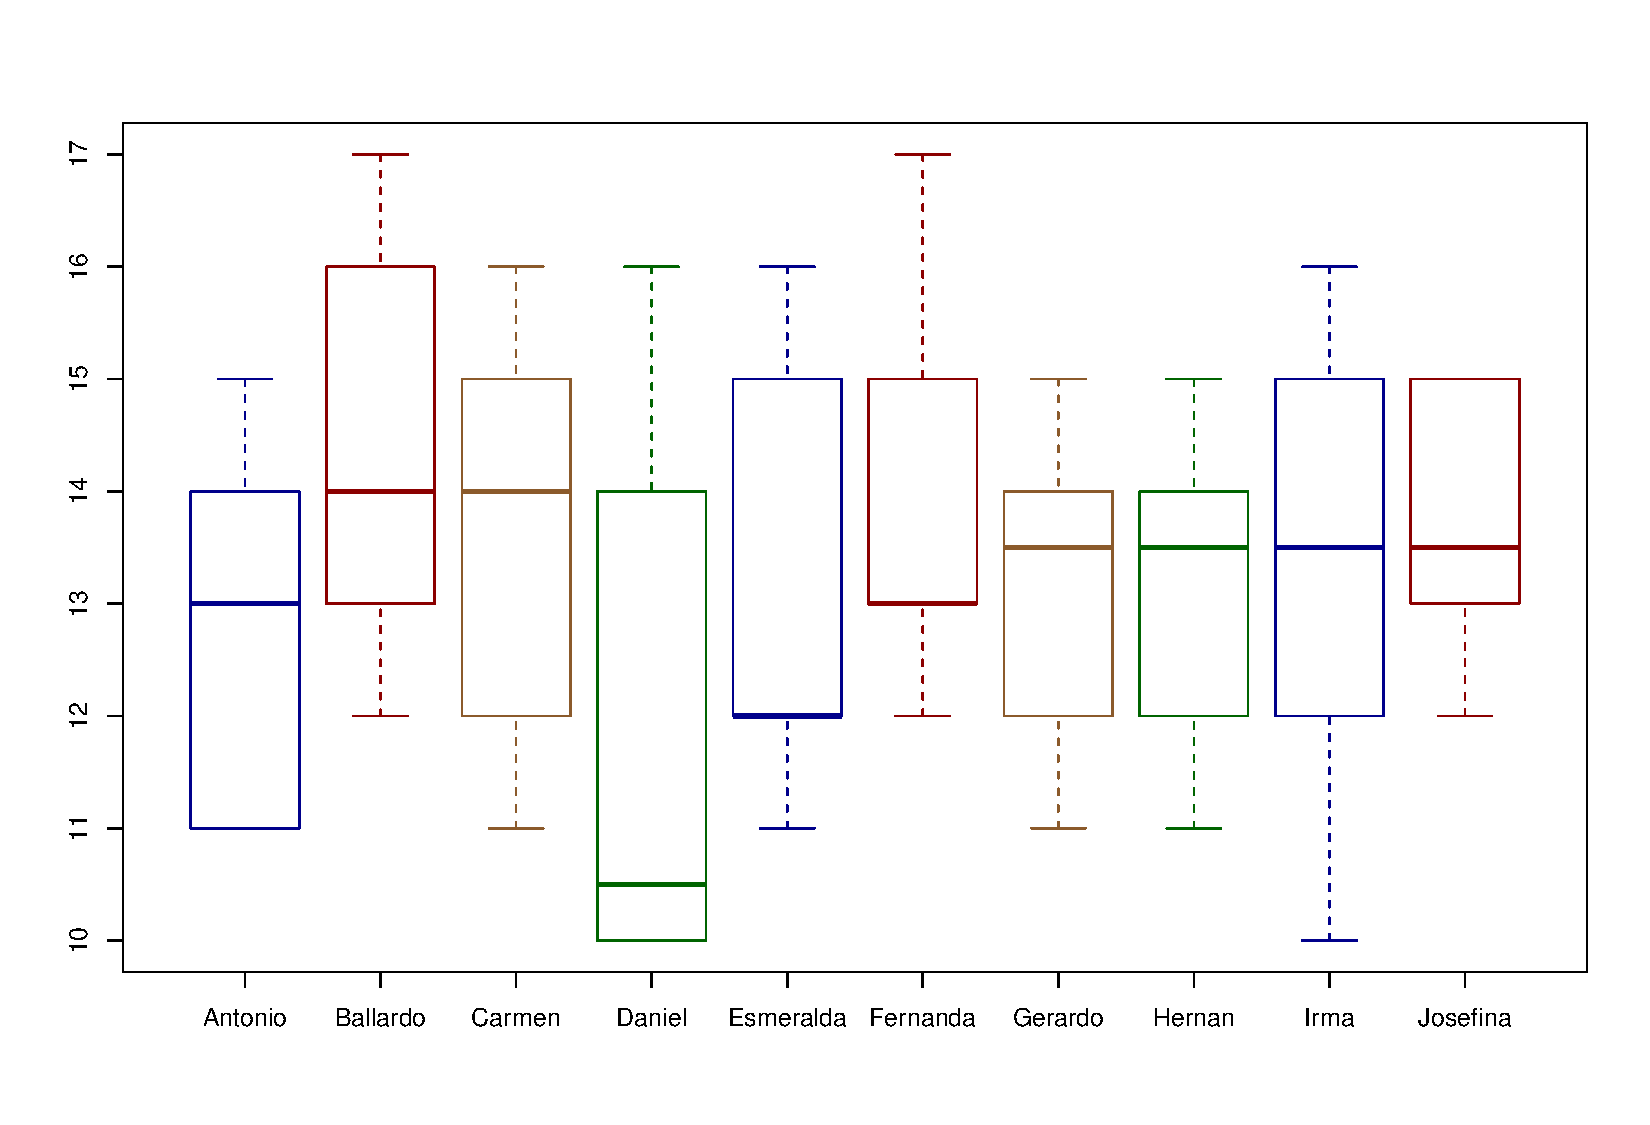
\includegraphics[scale=0.45]{99_05_bwJudge.pdf}
  \end{center}
\end{frame}

\begin{frame}
  Homoskedasticity of variances\\
  \vspace{0.5cm}
  \begin{minipage}[t]{0.48\textwidth}
    For each type of wine:\\

    \vspace*{0.25cm}
    Bartlett Test:\\
    \texttt{p value: 0.5726}\\

    \vspace*{0.75cm}
    Levene Test:\\
    \texttt{p value: 0.6283}\\
  \end{minipage}
  \hfill
  \begin{minipage}[t]{0.48\textwidth}
    For each judge:\\

    \vspace*{0.25cm}
    Bartlett Test:\\
    \texttt{p value: 0.9267}\\

    \vspace*{0.75cm}
    Levene Test:\\
    \texttt{p value: 0.9763}\\
  \end{minipage}
\end{frame}

\begin{frame}[fragile]
  \vspace{0.25cm}
  Variance analysis:
  \begin{verbatim}
            Df Sum Sq Mean Sq  F value   p value  
Wine         2  39.433 19.7167  7.0794 0.001794
Residuals   57 158.750  2.7851   
  \end{verbatim}
\end{frame}

\begin{frame}
   Graphical check of the model:\\
  \vspace{.1cm}
  \begin{center}
    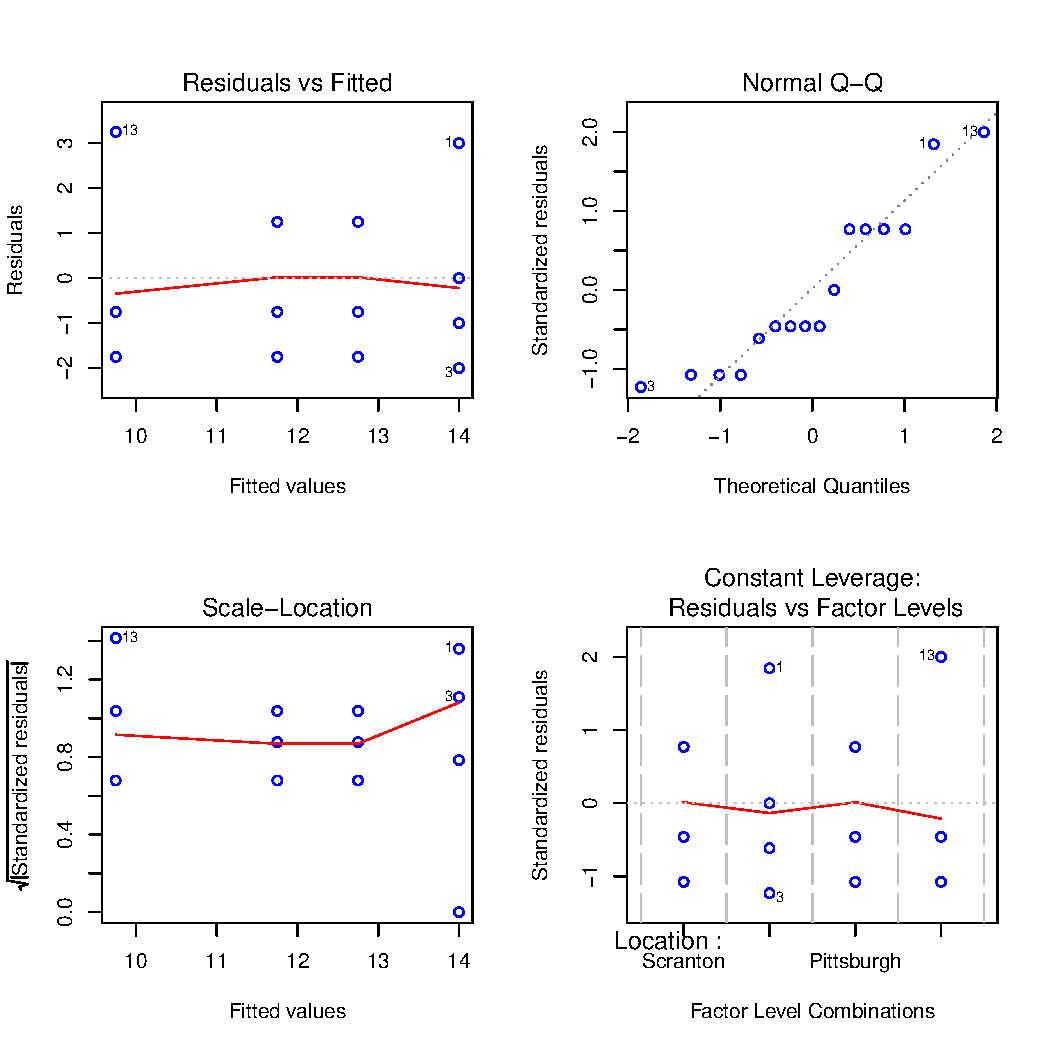
\includegraphics[width=7.5cm]{99_05_residAnovaPntWear1}
    \end{center}
\end{frame}

\begin{frame}[fragile]
  \vspace{0.25cm}
  Variance analysis:
  \begin{verbatim}
            Df Sum Sq Mean Sq  F value p value  
Judge        9  24.683  2.7426  0.7904 0.6264
Residuals   50 173.500  3.4700    
  \end{verbatim}
\end{frame}

\begin{frame}
   Graphical check of the model:\\
  \vspace{.1cm}
  \begin{center}
    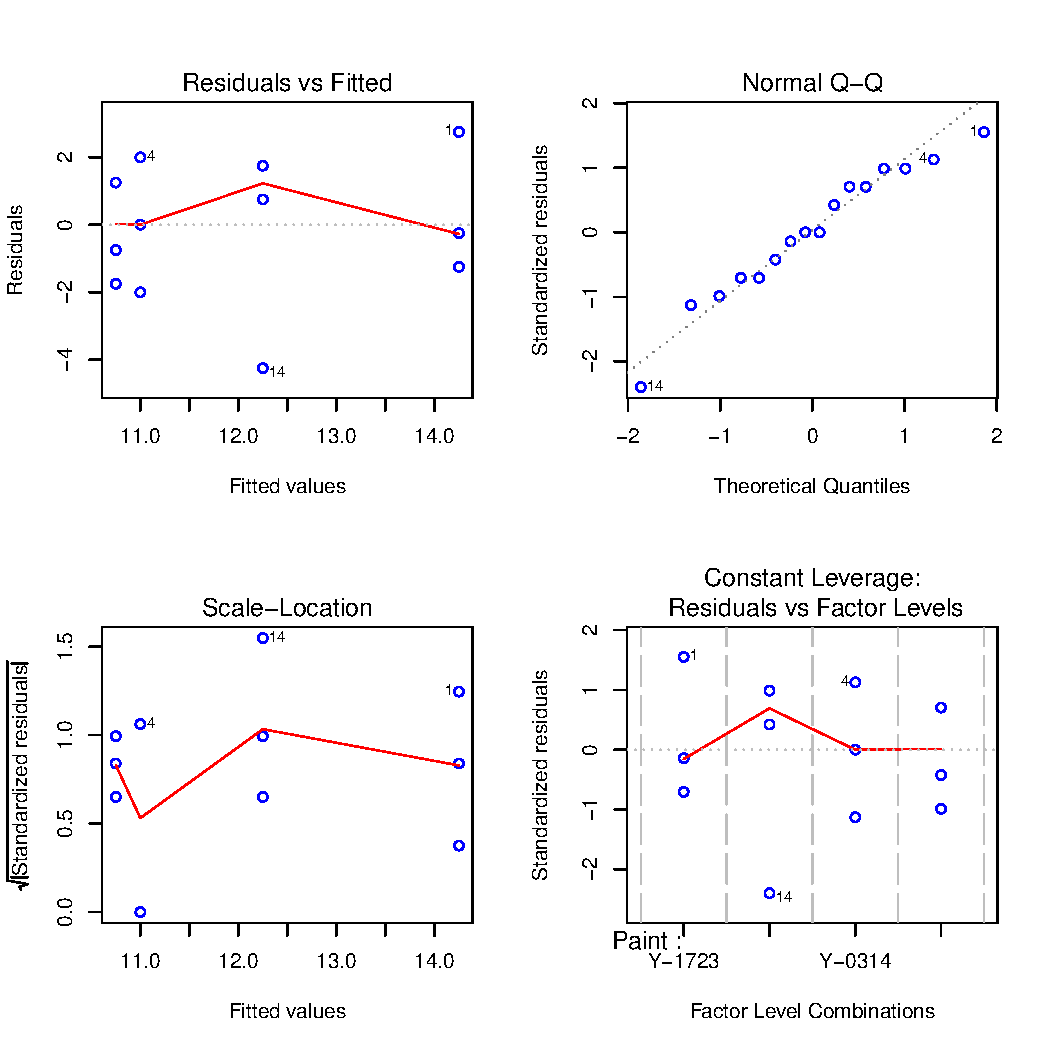
\includegraphics[width=7.5cm]{99_05_residAnovaPntWear2}
    \end{center}
\end{frame}

\begin{frame}[fragile]
  \vspace{0.25cm}
  Variance analysis:
  \begin{verbatim}
            Df Sum Sq Mean Sq  F value  p value   
Wine         2  39.433 19.7167  7.0592 0.002054
Judge        9  24.683  2.7426  0.9819 0.466912   
Residuals   48 134.067  2.7931    
  \end{verbatim}
\end{frame}

\begin{frame}
   Graphical check of the model:\\
  \vspace{.1cm}
  \begin{center}
    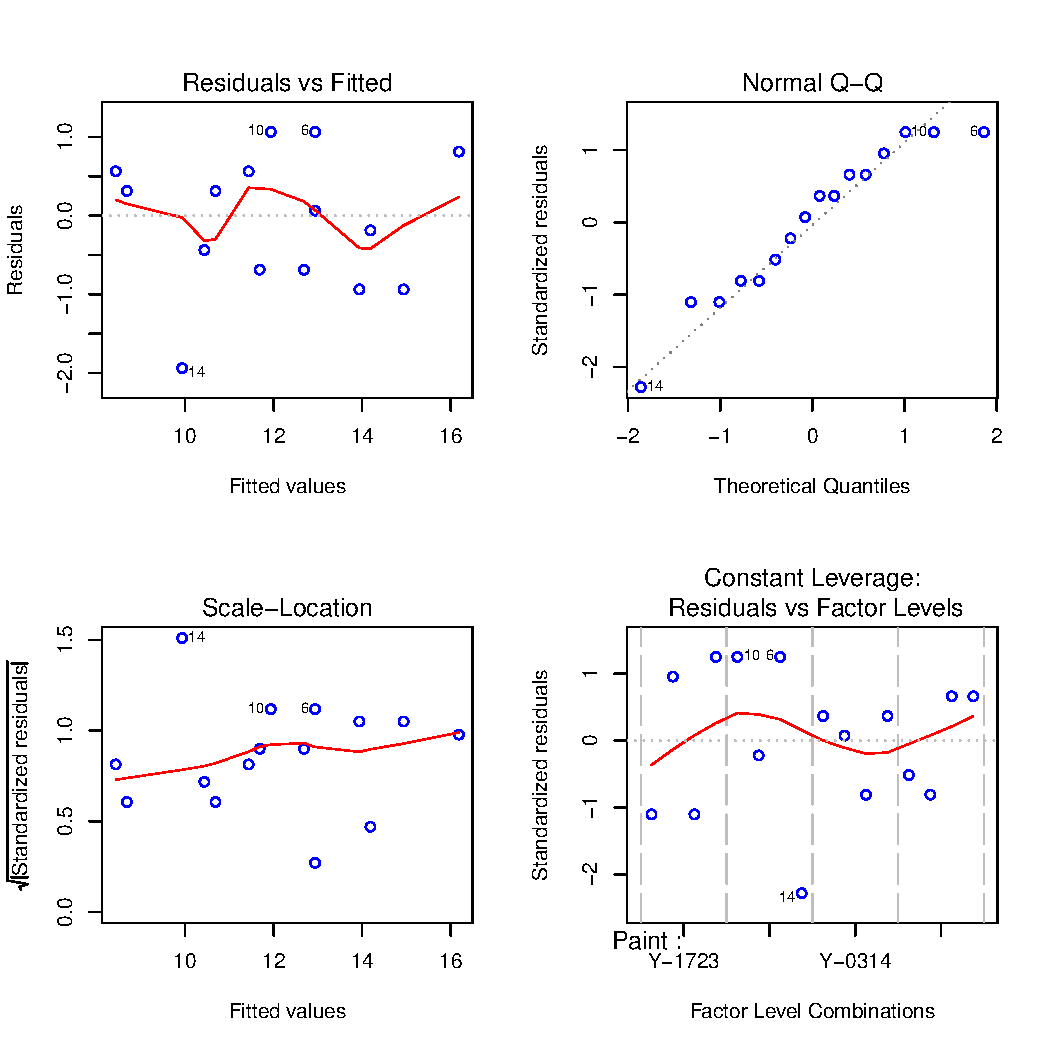
\includegraphics[width=7.5cm]{99_05_residAnovaPntWear3}
    \end{center}
\end{frame}

\livelloB{Wear of paint}

\begin{frame}
  \begin{description}
    \item[Data: ]pntwear.txt \\ 
    \item[Description: ]
      \begin{footnotesize}
        \begin{itemize}
          \item \textit{Location}: indicates the place of the test (factor);
          \item \textit{Paint}: indicates the type of paint (factor);
          \item \textit{PntWear}: indicates the wear of paint (score).
        \end{itemize}
      \end{footnotesize}
    \item[Aims: ]
      \begin{footnotesize}
        Pennsylvania Department of Transportation is studying the use of four different types of yellow paint for the street. The test is performed on the streets of Philadelphia, Pittsburgh, Harrisburg e Scranton, in Pennsylvania. After a period of exposure to the weather conditions and to the  traffic, the wear of paint is measured in the four cities. For the classification, a higher score was given to a lower wear of the paint. 
      \begin{itemize}
          \item[-] Let us perform an analysis of variance to check if the mean of the wear of the paint is equal for the four cities. 
          \item[-] Let us perform an analysis of variance to check if the mean of the wear of the paint is equal for the four types of paint. 
          \item[-] Let us perform an analysis of variance to check if the mean of the wear of the paint is different between the place and the type of paint.
        \end{itemize}
      \end{footnotesize}
  \end{description}
\end{frame}

\begin{frame}
  B-W Graph of \textit{PntWear} separately for each place:\\
  \begin{center}
    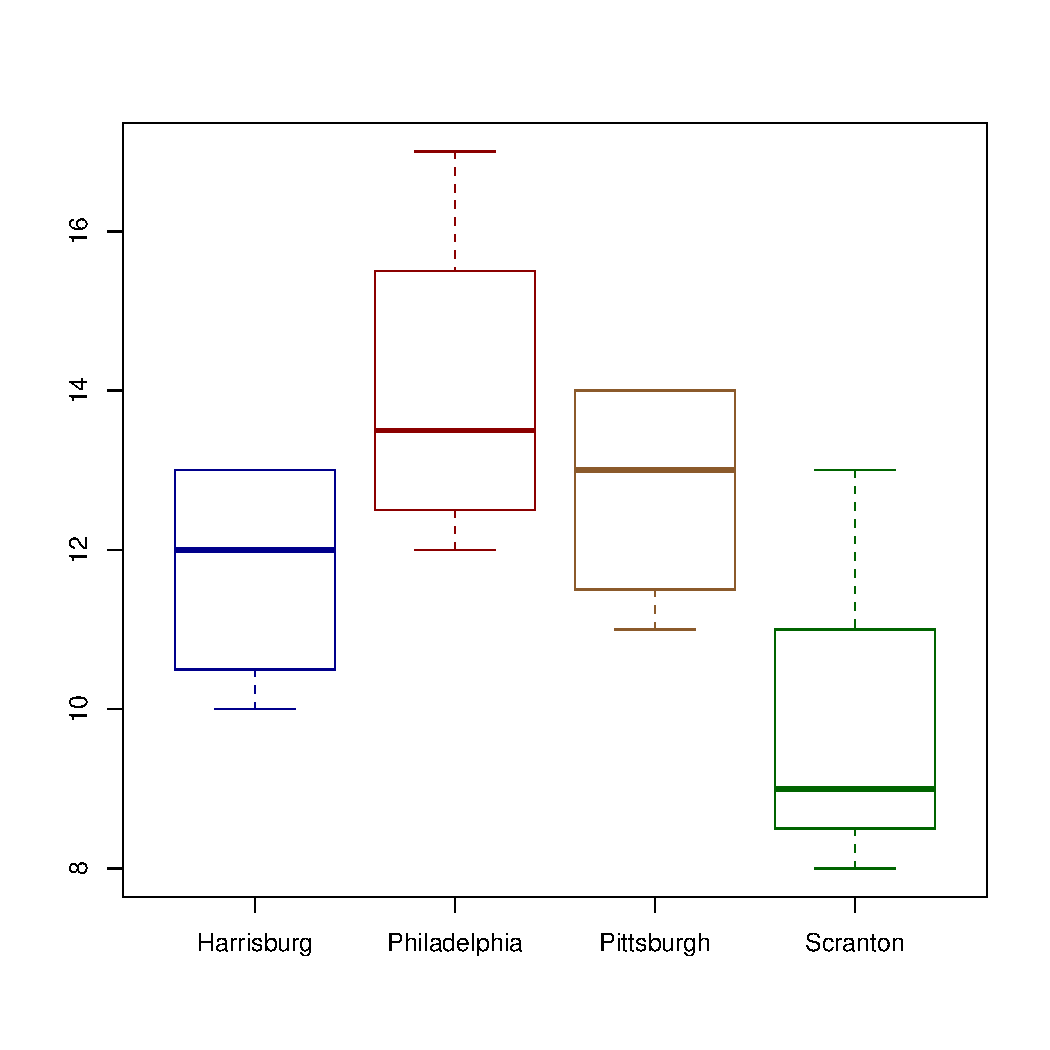
\includegraphics[width=7.5cm]{99_05_bwLocation.pdf}
  \end{center}
\end{frame}

\begin{frame}
  B-W Graph of \textit{PntWear} separately for each type of paint:\\
  \begin{center}
    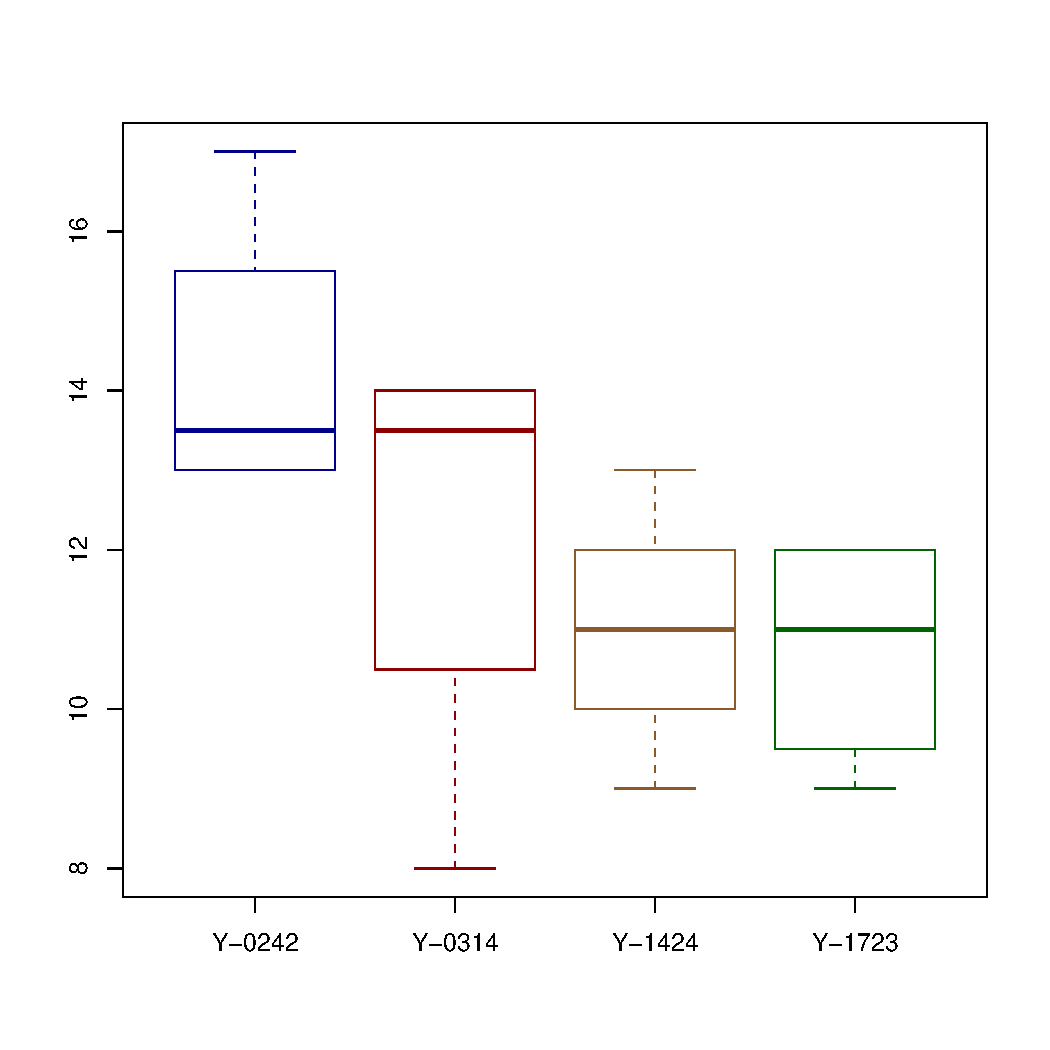
\includegraphics[width=7.5cm]{99_05_bwPaint.pdf}
  \end{center}
\end{frame}

\begin{frame}
  Homoskedasticity of variances\\
  \vspace{0.5cm}
  \begin{minipage}[t]{0.48\textwidth}
    For each place:\\

    \vspace*{0.25cm}
    Bartlett Test:\\
    \texttt{p value: 0.8644}\\

    \vspace*{0.75cm}
    Levene Test:\\
    \texttt{p value: 0.899}\\
  \end{minipage}
  \hfill
  \begin{minipage}[t]{0.48\textwidth}
    For each type of paint:\\

    \vspace*{0.25cm}
    Bartlett Test:\\
    \texttt{p value: 0.6940}\\

    \vspace*{0.75cm}
    Levene Test:\\
    \texttt{p value: 0.9231}\\
  \end{minipage}
\end{frame}

\begin{frame}[fragile]
  \vspace{0.25cm}
  Variance analysis:
  \begin{verbatim}
            Df Sum Sq Mean Sq F value p value  
Location     3 38.688 12.8958  3.6627 0.04404
Residuals   12 42.250  3.5208    
  \end{verbatim}
\end{frame}

\begin{frame}
   Graphical check of the model:\\
  \vspace{.1cm}
  \begin{center}
    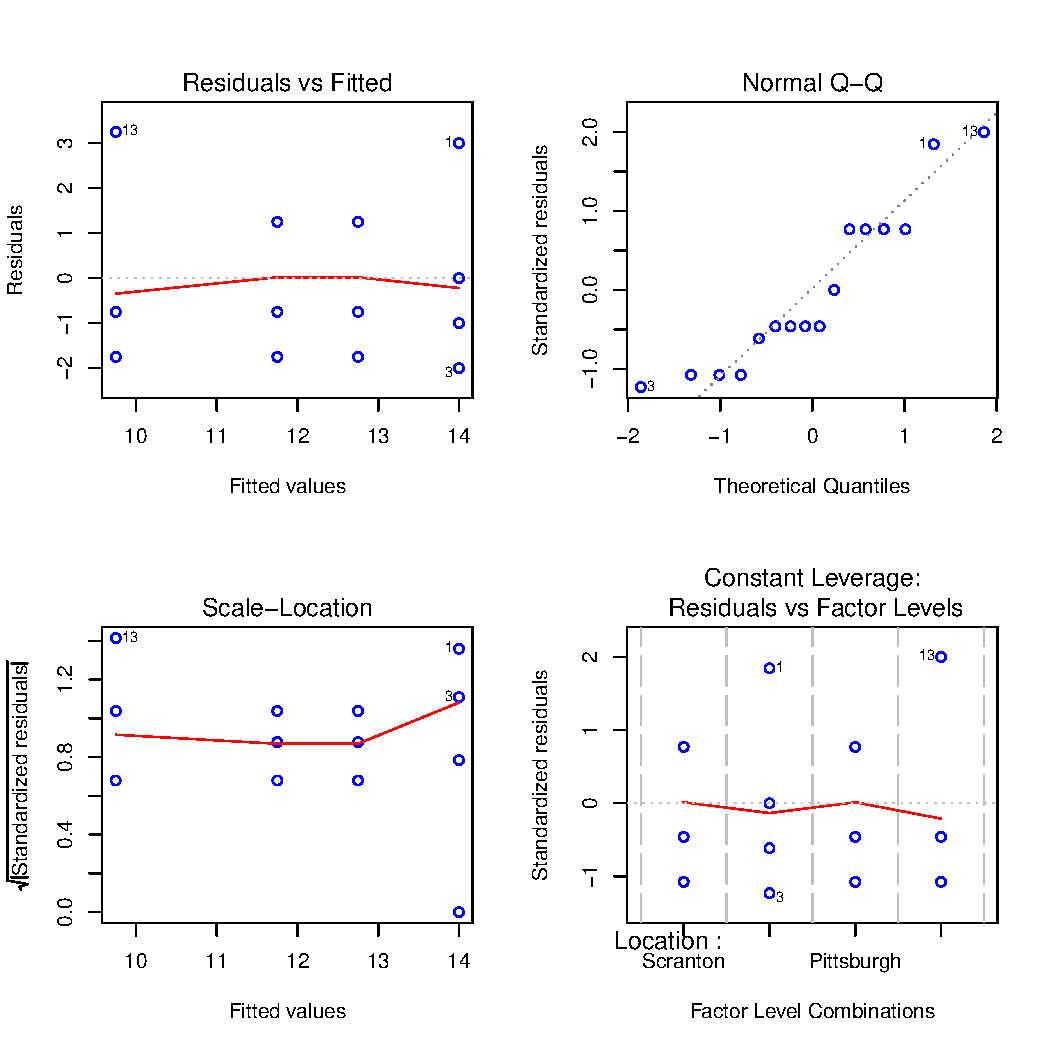
\includegraphics[width=7.5cm]{99_05_residAnovaPntWear1}
    \end{center}
\end{frame}

\begin{frame}[fragile]
  \vspace{0.25cm}
  Variance analysis:
  \begin{verbatim}
            Df Sum Sq Mean Sq F value p value  
Paint        3 30.688 10.2292  2.4428  0.1145
Residuals   12 50.250  4.1875     
  \end{verbatim}
\end{frame}

\begin{frame}
   Graphical check of the model:\\
  \vspace{.1cm}
  \begin{center}
    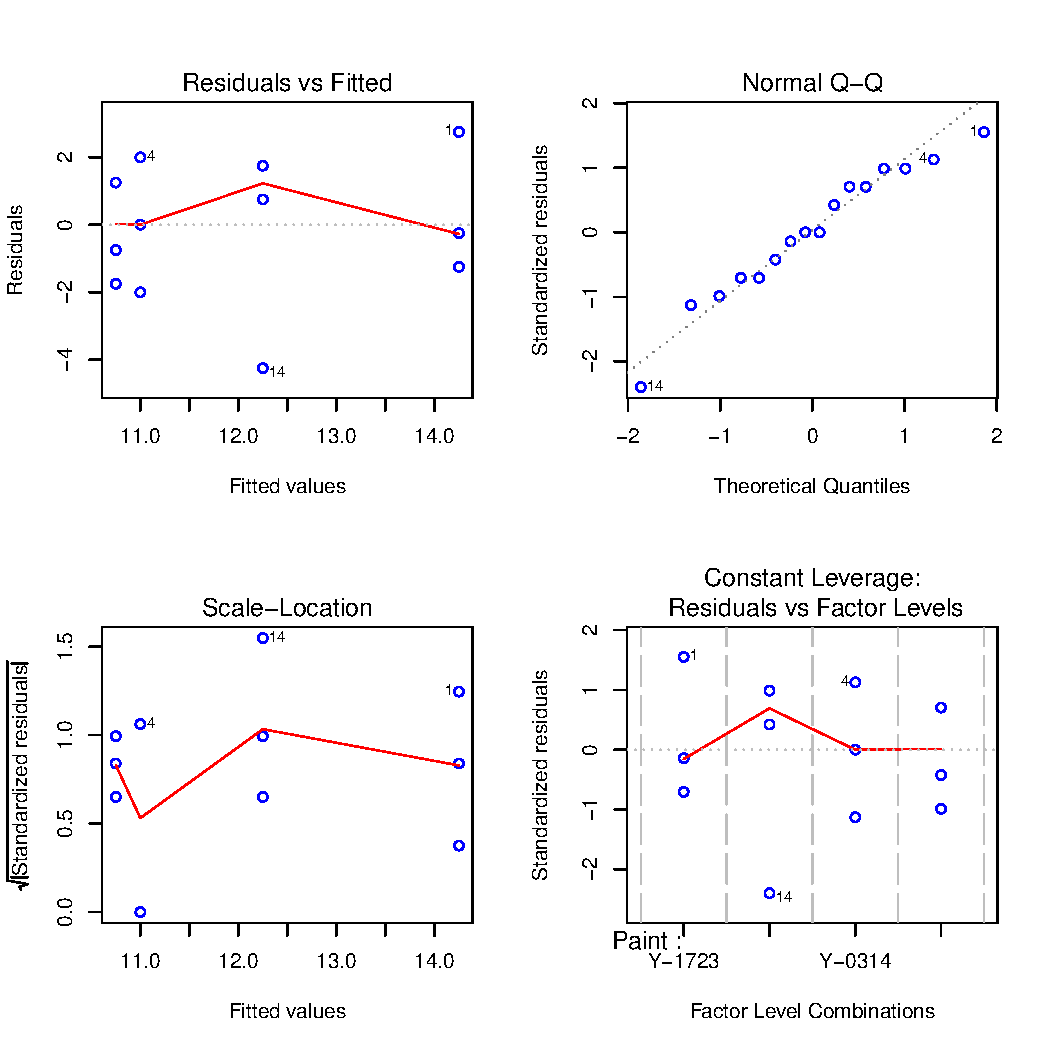
\includegraphics[width=7.5cm]{99_05_residAnovaPntWear2}
    \end{center}
\end{frame}

\begin{frame}[fragile]
  \vspace{0.25cm}
  Variance analysis:
  \begin{verbatim}
            Df Sum Sq Mean Sq F value  p value   
Paint        3 30.688 10.2292  7.9622 0.006685
Location     3 38.688 12.8958 10.0378 0.003133
Residuals    9 11.563  1.2847    
  \end{verbatim}
\end{frame}

\begin{frame}
   Graphical check of the model:\\
  \vspace{.1cm}
  \begin{center}
    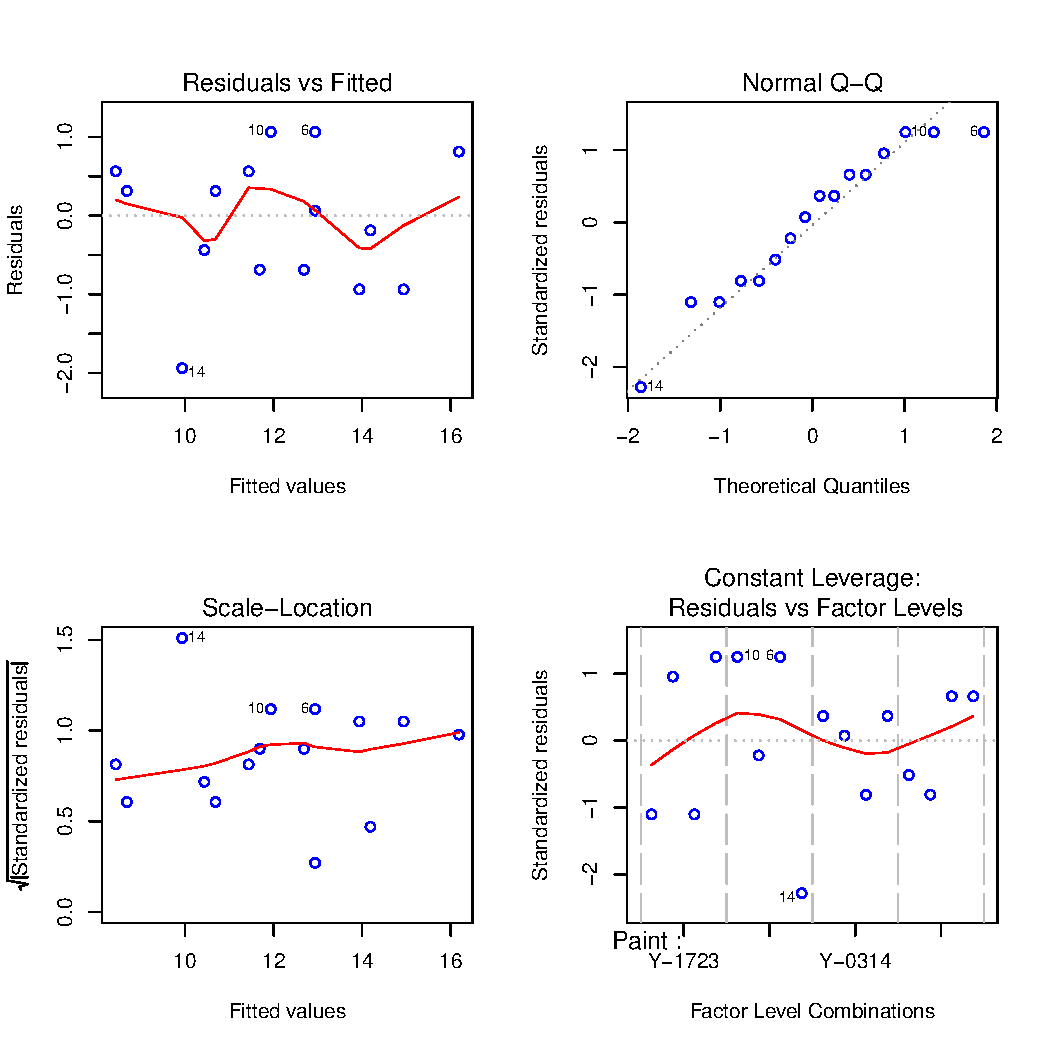
\includegraphics[width=7.5cm]{99_05_residAnovaPntWear3}
    \end{center}
\end{frame}



\livelloB{Penicillin production}

\begin{frame}
  \begin{description}
    \item[Data: ]penicillin.txt \\ 
    \item[Description: ]
      \begin{footnotesize}
        \begin{itemize}
          \item \textit{Mixture}: indicates the type of mixture chosen for the production (factor);
          \item \textit{Mode}: indicates the mode of production (factor);
          \item \textit{Penicillin}: indicates the quantity of penicillin produced.
        \end{itemize}
      \end{footnotesize}
    \item[Aims: ]
      \begin{footnotesize}
        The aim is to determine as the different modes of penicillin production (A, B, C, D) influence the quantity produced. Earlier It was observed that the mixture chosen for the production is rather variable and that this factor could somehow affect the production. So, It was decided to control also the effect of the mixture considering 5 mixtures (I, II, II, IV, V)  and using each of these in the four production processes. Let us note as in this case the interest is in the check if a difference of the effect on the quantities of penicillin produced with production mode exists, independently from the type of mixture used. 
      \end{footnotesize}
  \end{description}
\end{frame}

\begin{frame}
  \begin{description}
    \item[Aims: ]
      \begin{footnotesize}
        \begin{itemize}
          \item[-] Let us show the BW plot OF \textit{Penicillin} for each production mode and for each type of mixture.
          \item[-] By examining the BW plot, let us try to hypothesise if the modalities of production could detemine differences in the quantities of penicillin producted.
          \item[-] Performing an analysis of variance, let us check the hypothesis that the mode of production doesn't influence the quantity producted.
          \item[-] Let us look at what the differences may be due and let us repeat the analysis of variance considering the type of mixture.
        \end{itemize}
      \end{footnotesize}
  \end{description}
\end{frame}

\begin{frame}
  B-W Graph of \textit{Penicillin} for each mode of production:\\
  \vspace{-0.5cm}
  \begin{center}
    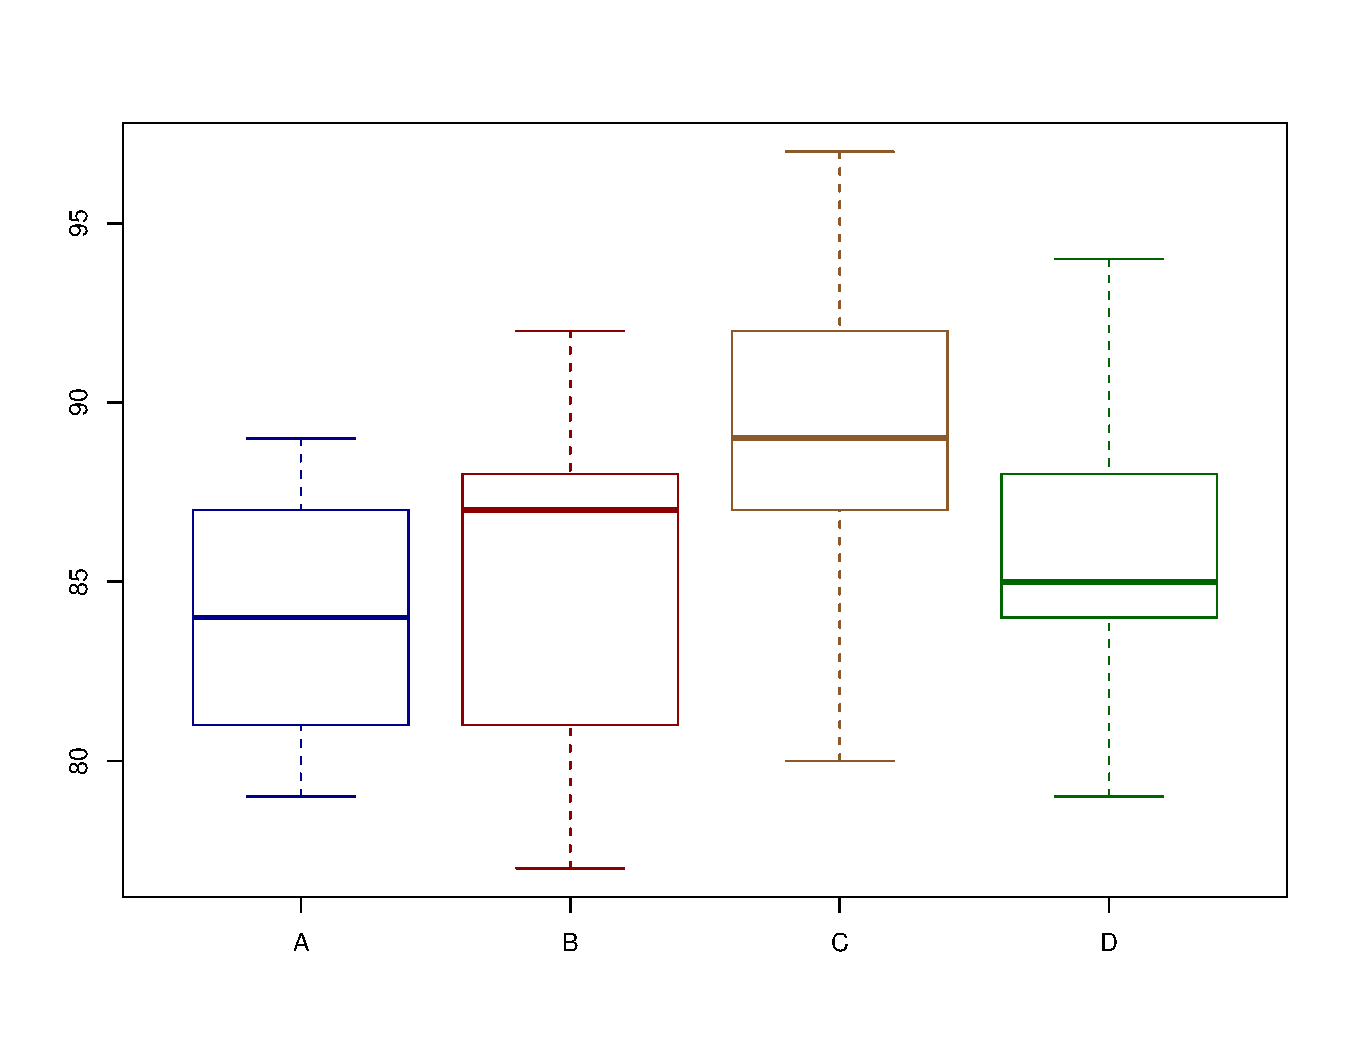
\includegraphics[width=11cm]{99_05_bwPenicillinMode.pdf}
  \end{center}
\end{frame}

\begin{frame}
  B-W Graph of \textit{Penicillin} for each type of mixture:\\
  \vspace{-0.5cm}
  \begin{center}
    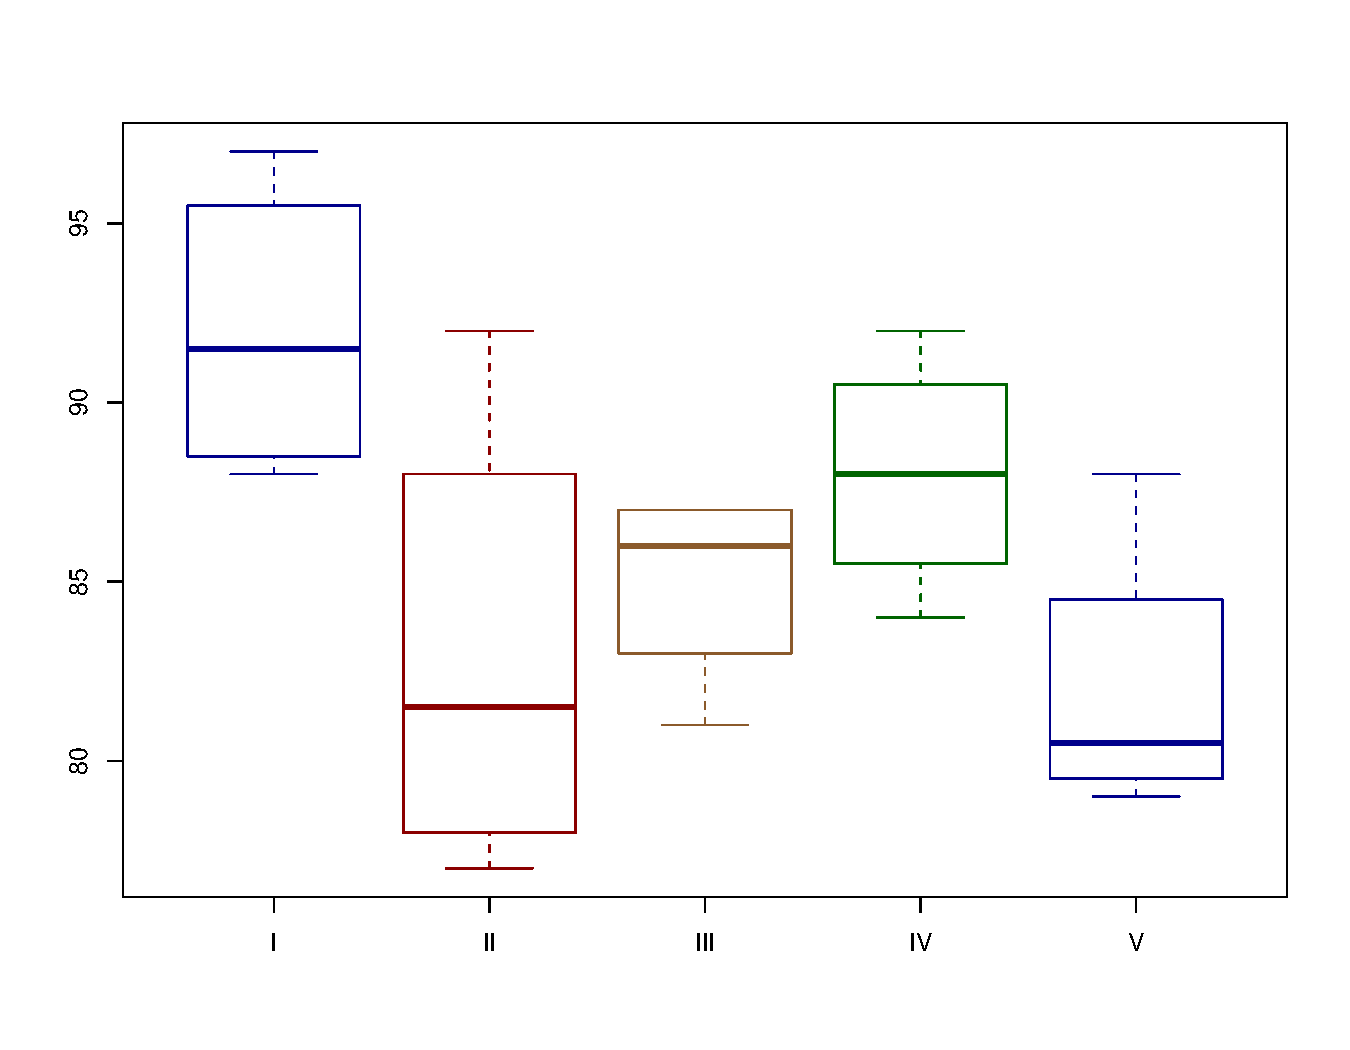
\includegraphics[width=11cm]{99_05_bwPenicillinMixture.pdf}
  \end{center}
\end{frame}

\begin{frame}
  Homoskedasticity of variances of \textit{Penicillin} for each mode of production\\
  \vspace*{0.25cm}
  Bartlett Test:\\
  \texttt{p value: 0.8755}\\
  \vspace*{0.25cm}
  Levene Test:\\
  \texttt{p value: 0.9388}\\
  \vspace*{0.75cm}
  Homoskedasticity of variances of \textit{Penicillin} for each type of mixture\\
  \vspace*{0.25cm}
  Bartlett Test:\\
  \texttt{p value: 0.6652}\\
  \vspace*{0.25cm}
  Levene Test:\\
  \texttt{p value: 0.5311}\\
\end{frame}

\begin{frame}[fragile]
  \vspace{0.25cm}
  Variance analysis (model that does not consider the type of mixture):
  \begin{verbatim}  
            Df Sum Sq Mean Sq F value p value
Mode         3     70  23.333  0.7619  0.5318
Residuals   16    490  30.625     
  \end{verbatim}
  \vspace{0.25cm}
  Variance analysis (model that consider the type of mixture):
  \begin{verbatim}  
            Df Sum Sq Mean Sq F value p value  
Mode         3     70  23.333  1.2389 0.33866  
Mixture      4    264  66.000  3.5044 0.04075
Residuals   12    226  18.833     
  \end{verbatim}
\end{frame}

\begin{frame}
   Graphical check of the model:\\
  \vspace{.1cm}
  \begin{center}
    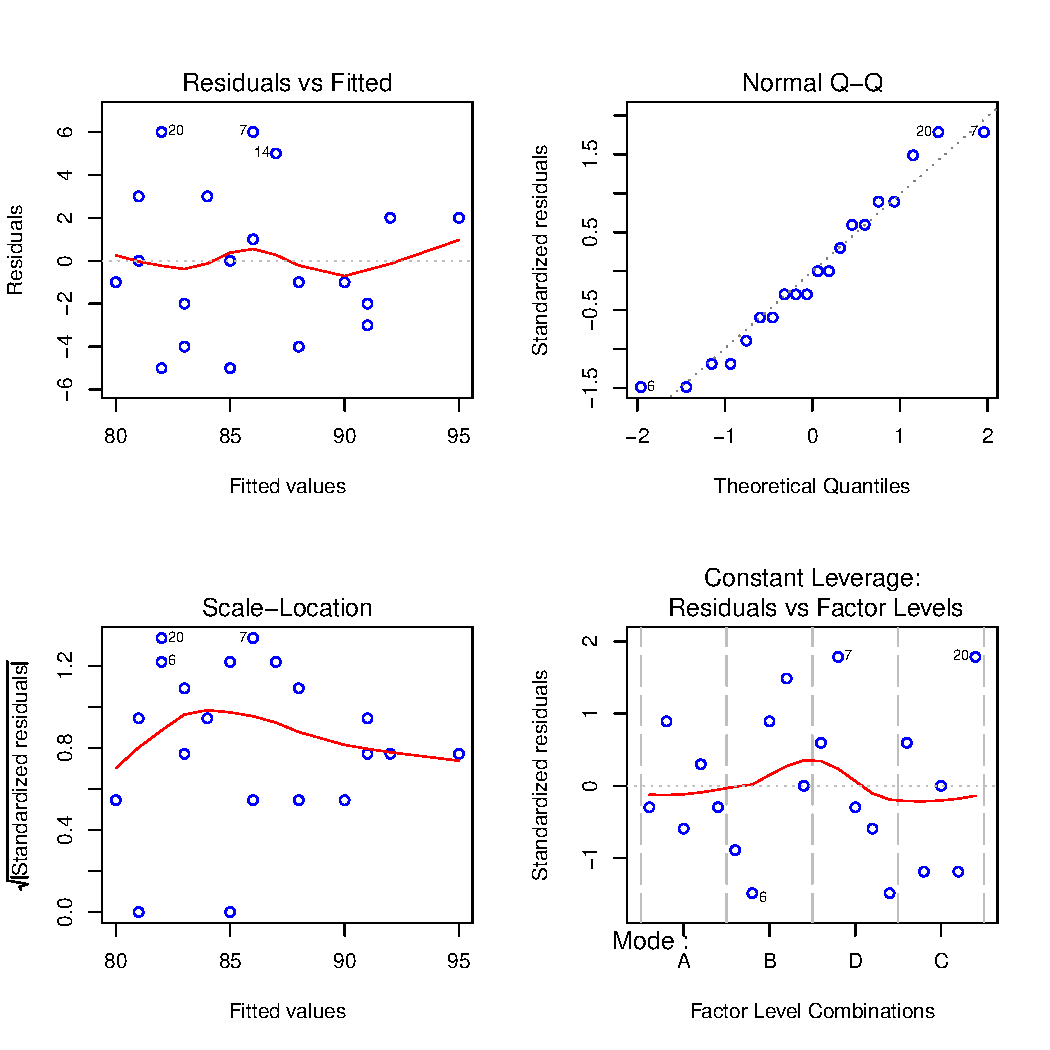
\includegraphics[width=7.5cm]{99_05_residAnovaPenicillin}
    \end{center}
\end{frame}


\livelloB{Effect of toxic agent}

\begin{frame}
  \begin{description}
    \item[Data: ]rats.txt \\ 
    \item[Description: ]
      \begin{footnotesize}
        \begin{itemize}
          \item \textit{Time}: identifies the survival time (in tens of hours);
          \item \textit{Poison}: identifies the poison type (factor);
          \item \textit{Treatment}: identifies the type of treatment (factor).
        \end{itemize}
      \end{footnotesize}
    \item[Aims: ]
      \begin{footnotesize}
        Let us consider three types of poison and four types of treatment. Each combination poison-treatment is administered to four rats. 
        \begin{itemize}
          \item[-] Let us show BW plot OF \textit{Time} for each type of poison.
          \item[-] Let us transform the variable \textit{Time} in its reciprocal.
          \item[-] Let us check the presence of the interaction effect between poison and type of treatment.
        \end{itemize}
      \end{footnotesize}
  \end{description}
\end{frame}

\begin{frame}
  B-W Graph of \textit{Time} separately for each type of poison:\\
  \vspace{-0.5cm}
  \begin{center}
    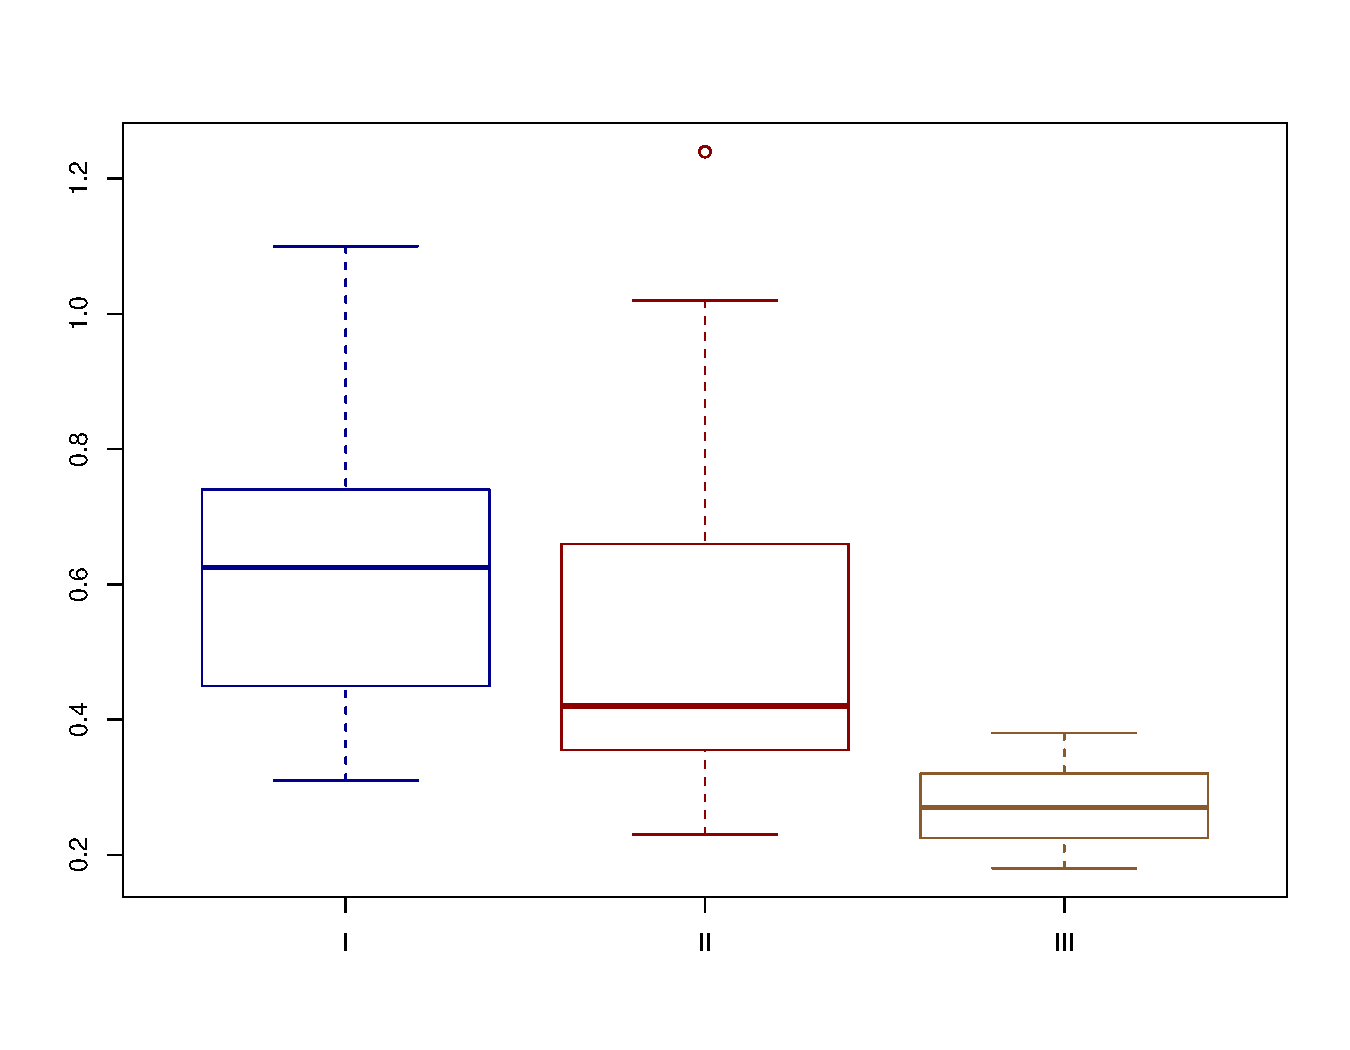
\includegraphics[width=11cm]{99_05_bwPoison.pdf}
  \end{center}
\end{frame}

\begin{frame}
  B-W Graph for the reciprocal of \textit{Time} for each type of poison:\\
  \vspace{-0.5cm}
  \begin{center}
    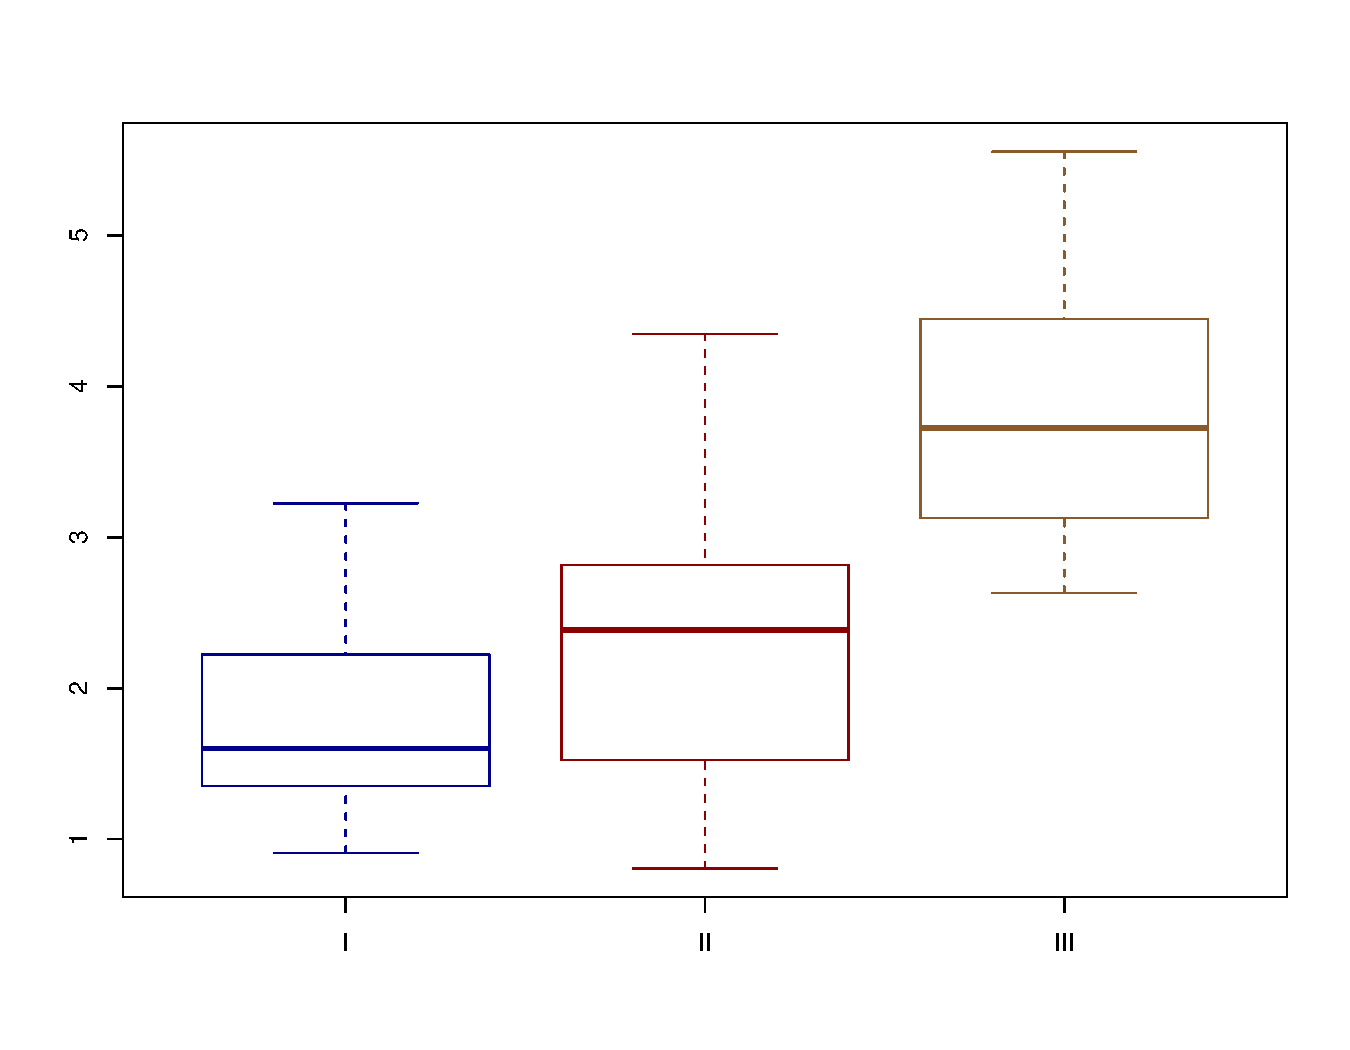
\includegraphics[width=11cm]{99_05_bwInvPoison.pdf}
  \end{center}
\end{frame}

\begin{frame}
  Normality\\
  \vspace*{0.25cm}
  Because of the low number of units within each groups, It is not possible to perform Anderson Darling test. However, analysing the B-W plot of the previous slide, the normality assumption is considered valid. \\
  \vspace{1cm}
  Homoskedasticity of variances of the reciprocal of \textit{Time} for each type of poison\\
  \vspace*{0.25cm}
  Bartlett Test:\\
  \texttt{p value: 0.2105}\\
  \vspace*{0.75cm}
  Levene Test:\\
  \texttt{p value: 0.1915}\\
\end{frame}

\begin{frame}[fragile]
  \vspace{0.25cm}
  Variance analysis (model with interaction):
  \begin{verbatim}  
                 Df Sum Sq Mean Sq F value   p value   
Treatment         3 20.414  6.8048 28.3431 1.376e-09
Poison            2 34.877 17.4386 72.6347 2.310e-13
Treatment:Poison  6  1.571  0.2618  1.0904    0.3867    
Residuals        36  8.643  0.2401      
  \end{verbatim}
  \vspace{0.25cm}
  Variance analysis (model without interaction):
  \begin{verbatim}  
            Df Sum Sq Mean Sq F value   p value    
Treatment    3 20.414  6.8048  27.982 4.192e-10
Poison       2 34.877 17.4386  71.708 2.865e-14
Residuals   42 10.214  0.2432      
  \end{verbatim}
\end{frame}

\begin{frame}
   Graphical check of the model:\\
  \vspace{.1cm}
  \begin{center}
    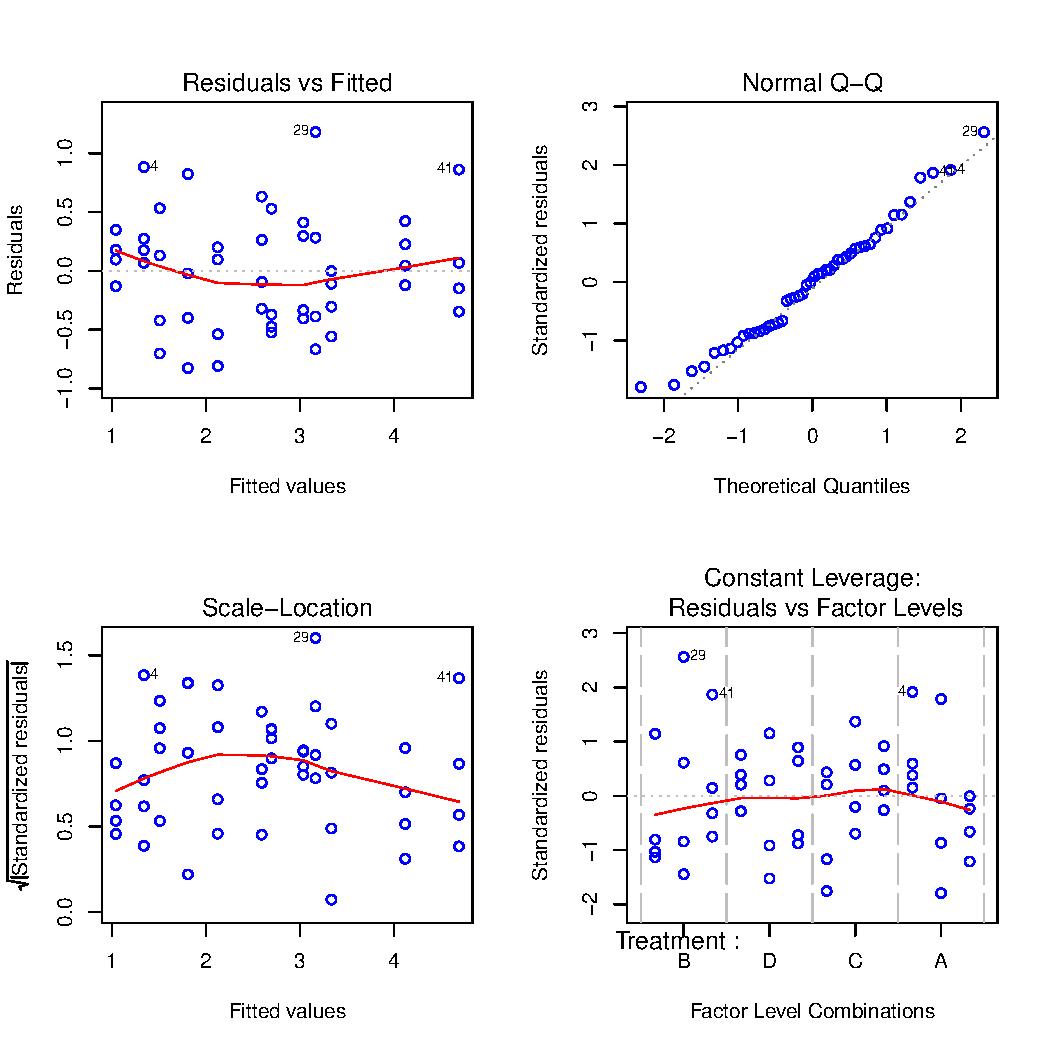
\includegraphics[width=7.5cm]{99_05_residAnovaInvTreatmentPoison}
    \end{center}
\end{frame}

\livelloB{Solvent for varnish}

\begin{frame}
  \begin{description}
    \item[Data: ]varnish.txt \\ 
    \item[Description: ]
      \begin{footnotesize}
        \begin{itemize}
          \item \textit{Solvent}: indicates the type of solvent (factor);
          \item \textit{Varnish}: indicates the type of varnish (factor);
          \item \textit{Time}: indicates the time necessary to dissolve the stain (minutes).
        \end{itemize}
      \end{footnotesize}
    \item[Aims: ]
      \begin{footnotesize}
        The aim is to evaluate the efficacy of a solvent to dissolve stains of nail varnish from fabrics. It is used two types of solvent and three types of varnish. The experiment consists of immersing 5 stained fabrics by a certain type of varnish into a bowl with a solvent, measuring the time (in minutes) necessary to dissolve the stain. 
        \begin{itemize}
          \item[-] Let us evaluate also if there are differences in the types of solvent in respect of the types varnish that produced the stain.
        \end{itemize}
      \end{footnotesize}
  \end{description}
\end{frame}

\begin{frame}
  B-W Graph of \textit{Time} separately for each type of solvent:\\
  \vspace{-0.5cm}
  \begin{center}
    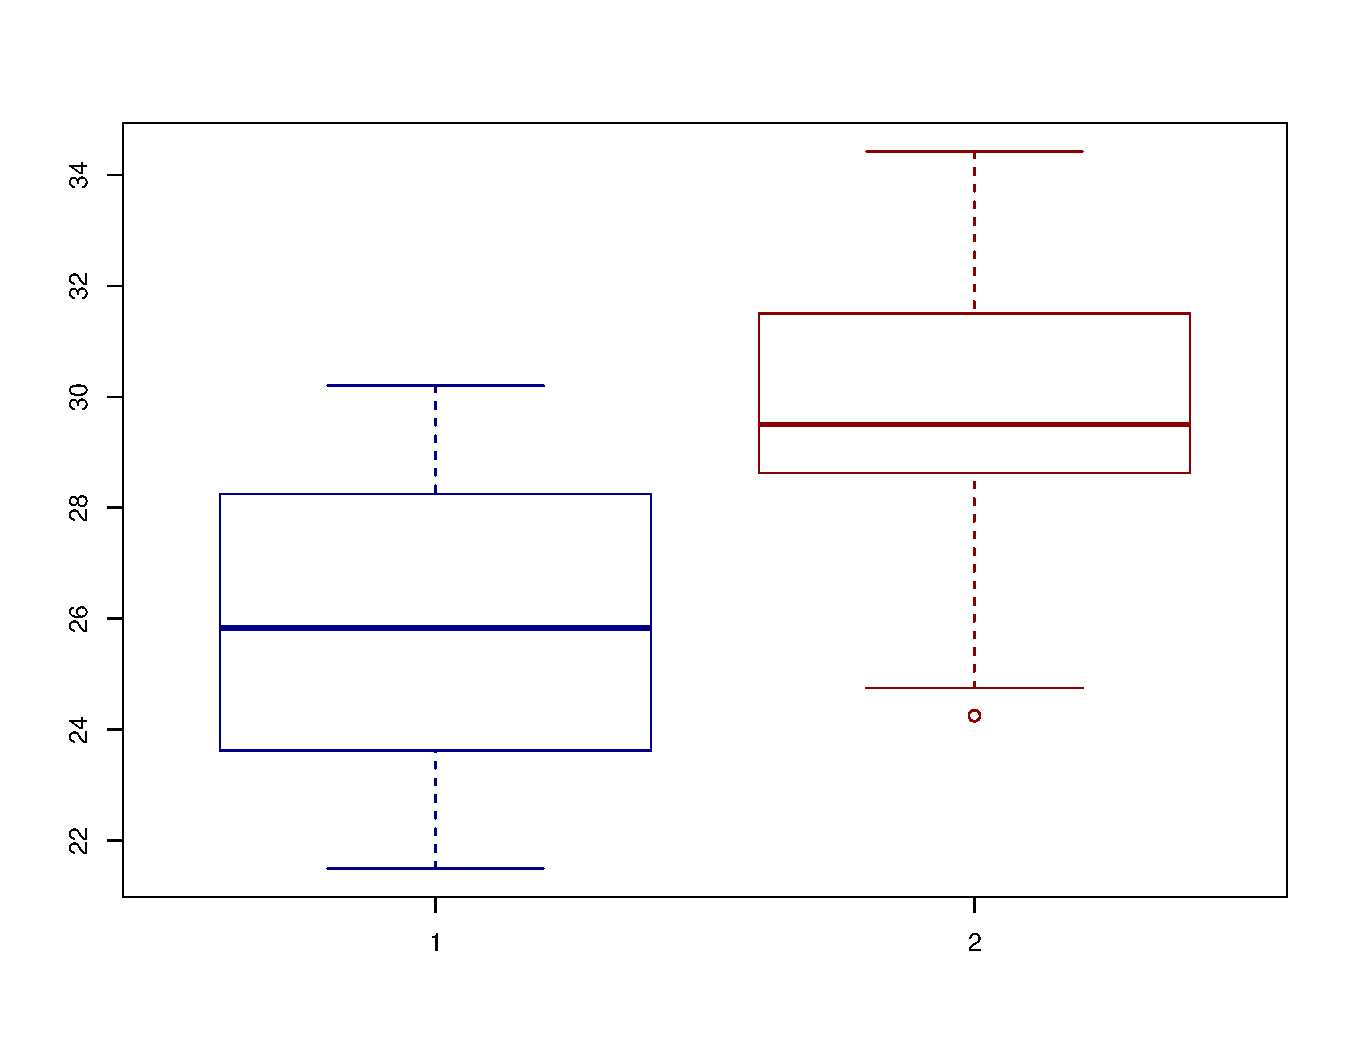
\includegraphics[width=11cm]{99_05_bwVarnishSolvent.pdf}
  \end{center}
\end{frame}

\begin{frame}
  B-W Graph of the reciprocal of \textit{Time} for each type of varnish:\\
  \vspace{-0.5cm}
  \begin{center}
    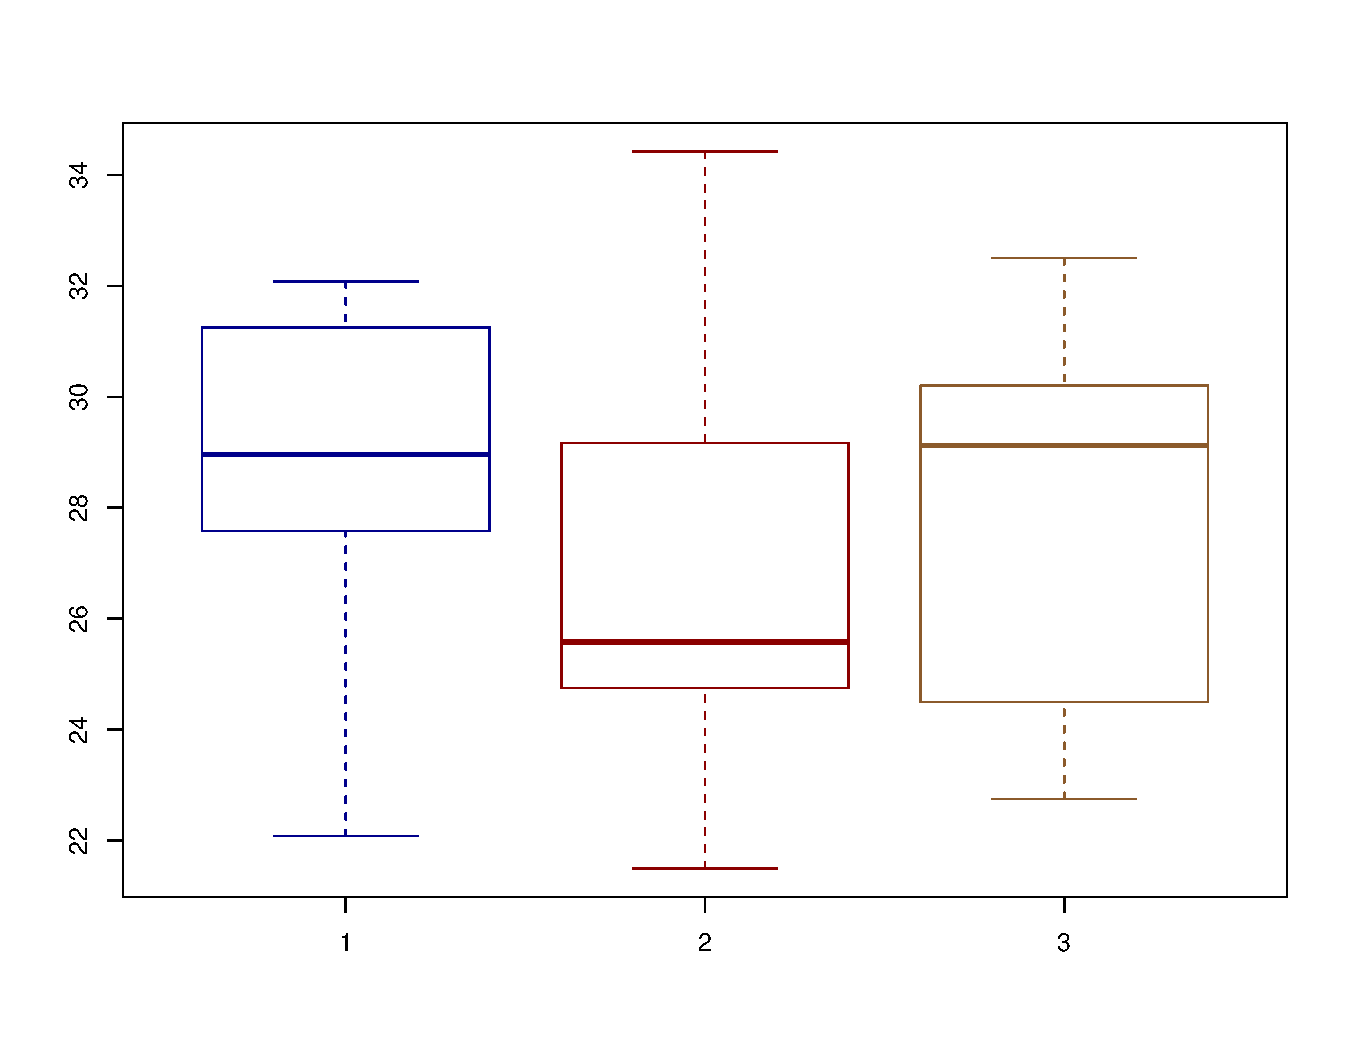
\includegraphics[width=11cm]{99_05_bwVarnishVarnish.pdf}
  \end{center}
\end{frame}

\begin{frame}
  Normality\\
  \vspace*{0.25cm}
  Anderson-Darling test doesn't reject the hypothesis of normality of \textit{Time} separately for each type of solvent and of \textit{Time} separately for each type of varnish.\\
  \vspace{1cm}
  Homoskedasticity of variances\\
  \vspace*{0.25cm}
  Both levene and Bartlett test doesn't reject the hypothesis of the homoskedasticity of \textit{Time}separately for each type of solvent and of \textit{Time}separately for each type of varnish.\\    
\end{frame}

\begin{frame}[fragile]
  \vspace{0.25cm}
  Variance analysis (complete model):
  \begin{verbatim}  
                Df  Sum Sq Mean Sq F value  p value   
Varnish          2  18.636   9.318  1.0695 0.358990   
Solvent          1  97.416  97.416 11.1810 0.002706
Varnish:Solvent  2   7.673   3.836  0.4403 0.648930   
Residuals       24 209.104   8.713  
  \end{verbatim}
  \vspace{0.25cm}
  Variance analysis (model which considers only the type of solvent):
  \begin{verbatim}  
            Df  Sum Sq Mean Sq F value  p value
Solvent      1  97.416  97.416  11.587 0.002022
Residuals   28 235.412   8.408      
  \end{verbatim}
\end{frame}

\begin{frame}
   Graphical check of the model:\\
  \vspace{.1cm}
  \begin{center}
    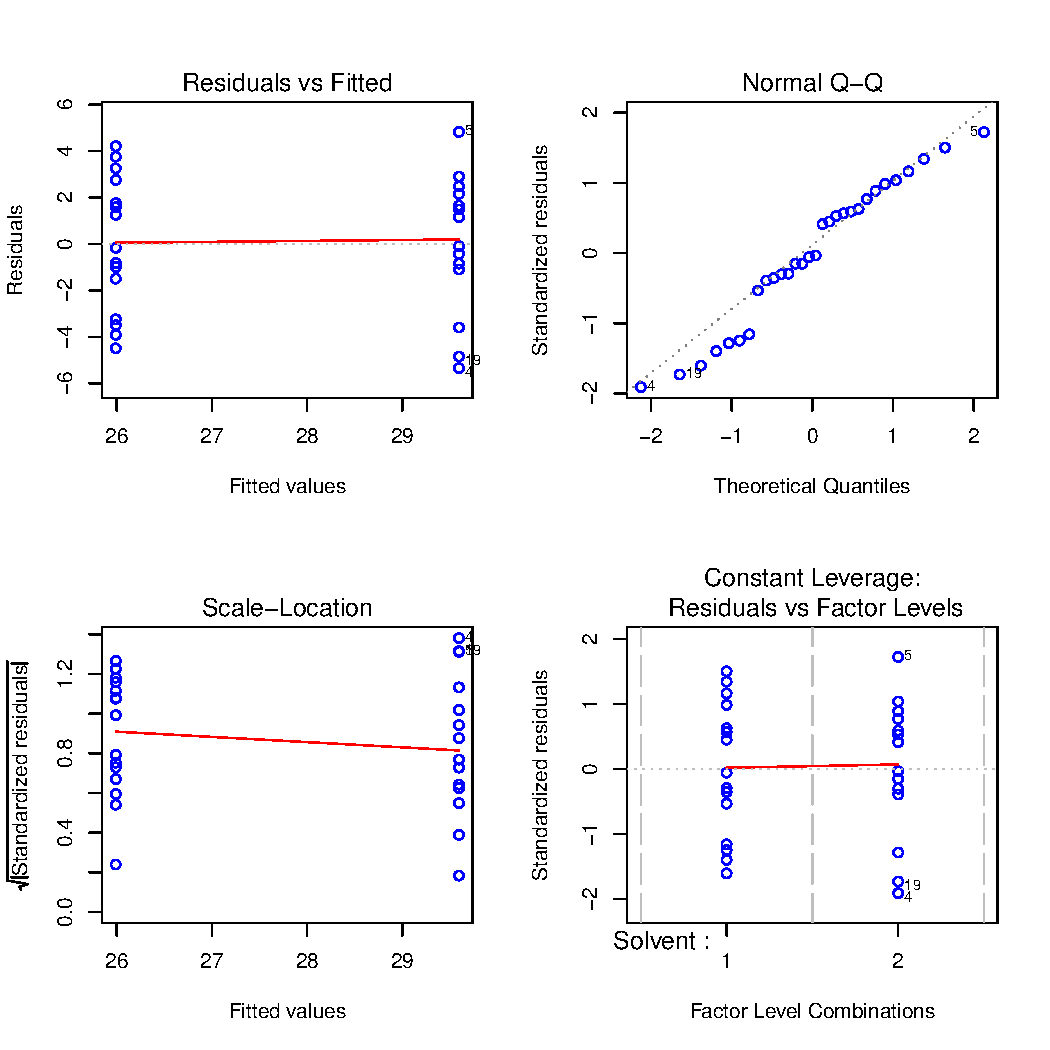
\includegraphics[width=7.5cm]{99_05_residAnovaVarnish}
    \end{center}
\end{frame}
